\documentclass[
 reprint,
 amsmath,amssymb,
 aps,
]{revtex4-1}

\usepackage{graphicx}  
\usepackage{epstopdf}
\usepackage{dcolumn}
\usepackage{bm}	
\usepackage{amsmath}		
\usepackage{amsfonts}			
\usepackage{amssymb}			
\usepackage{latexsym}		
\usepackage{color}
\usepackage{ stmaryrd }
\usepackage[utf8]{inputenc}
\usepackage[english]{babel}

\def\tc{\textcolor{red}}
\begin{document}

\title{ 
Forward scattering of a plane wave and of a spatially smoothed laser pulse  in the hydrodynamic and kinetic frameworks }
\author{C. Ruyer}\email{charles.ruyer@cea.fr}
\affiliation{CEA, DAM, DIF, F-91297 Arpajon, France}
\author{A. Debayle}
\affiliation{CEA, DAM, DIF, F-91297 Arpajon, France}
\author{M. Casanova}
\affiliation{CEA, DAM, DIF, F-91297 Arpajon, France}
\author{J. Fuchs}
\affiliation{LULI - CNRS, CEA, UPMC Univ Paris 06: Sorbonne Universit\'e, Ecole Polytechnique, Institut Polytechnique de Paris - F-91128 Palaiseau Cedex, France}
\author{J. R. Marqu\`{e}s}
\affiliation{LULI - CNRS, CEA, UPMC Univ Paris 06: Sorbonne Universit\'e, Ecole Polytechnique, Institut Polytechnique de Paris - F-91128 Palaiseau Cedex, France}
\author{L. Romagnani}
\affiliation{LULI - CNRS, CEA, UPMC Univ Paris 06: Sorbonne Universit\'e, Ecole Polytechnique, Institut Polytechnique de Paris - F-91128 Palaiseau Cedex, France}
\author{P. Antici}
%\footnote{present address: INRS-EMT, 1650, boulevard Lionel-Boulet, J3X 1S2, Varennes (Québec), Canada}
\altaffiliation[present address: ]{INRS-EMT, 1650, boulevard Lionel-Boulet, J3X 1S2, Varennes (Qu\'ebec), Canada}
\affiliation{LULI - CNRS, CEA, UPMC Univ Paris 06: Sorbonne Universit\'e, Ecole Polytechnique, Institut Polytechnique de Paris - F-91128 Palaiseau Cedex, France}
\author{N. Bourgeois}
\altaffiliation[present address: ]{Central Laser Facility, STFC Rutherford Appleton Laboratory, Didcot OX11 0QX, United Kingdom}
\affiliation{LULI - CNRS, CEA, UPMC Univ Paris 06: Sorbonne Universit\'e, Ecole Polytechnique, Institut Polytechnique de Paris - F-91128 Palaiseau Cedex, France}
\author{M. Nakatsutsumi}
\altaffiliation[present address: ]{European XFEL, GmbH, Holzkoppel 4, 22869 Schenefeld, Germany}
%\footnote{present address: European XFEL, GmbH, Holzkoppel 4, 22869 Schenefeld, Germany}
\affiliation{Institute of Laser Engineering, Osaka University, 02-06 Yamada-Oka, Suita, Osaka, 565-0871, Japan}
\author{M. Safronova}
\affiliation{Institute of Applied Physics, RAS, 46 Ulyanov Street, 603950 Nizhny Novgorod, Russia}
\author{M. Starodubtsev}
\affiliation{Institute of Applied Physics, RAS, 46 Ulyanov Street, 603950 Nizhny Novgorod, Russia}
\author{P. Loiseau}
\affiliation{CEA, DAM, DIF, F-91297 Arpajon, France}
\author{P. E. Masson-Laborde}
\affiliation{CEA, DAM, DIF, F-91297 Arpajon, France}
\author{T. Lin}
\affiliation{Fox Chase Cancer Center
333 Cottman Avenue
Philadelphia, PA 19111, USA} 

\begin{abstract}
We address the scattering of a high energy laser pulse on a   large wavelength acoustic turbulence of relevance for LMJ or NIF-class  experiments. 
Both kinetic and hydrodynamic frameworks are adopted and combined with a linearized  description of the laser propagation. The resulting dispersion relations display important kinetic  contributions to the growth of the Forward Brillouin instability.  
Moreover, proof is made that the optical smoothing techniques  often used in high energy laser facilities are, for cold enough plasmas or in the multi ion species case, not enough to reach full control of the laser filamentation.
Comparisons with experimental results and dedicated hydrodynamic %and particle-in-cell
simulations confirm our results. 
The   derived dispersion relations  present unique tools for assessing the propagation quality and energy deposition region of high energy lasers pulses. They also underlines the importance of accounting correctly for kinetic effects, even in the millimeters and nanoseconds scales of many  ICF or high-energy-density experiments. 
\end{abstract}

\maketitle 

\section{Introduction}
%\begin{itemize}
   % \item It requires the precise predictions of the  laser propagation along with parametric instabilities and their coupling with the smoothing technics, routinely used in high energy class facilities \cite[]{NatPhys_Glenzer,NatPhys_Labaune}.  
    %\item Forward instabilities such as filamentation \cite[]{phd_Michel,POP_michel_2003,Lushnikov_2006,PRL_Sarri_2011}, forward Brillouin  or plasma smoothing effects \cite[]{phd-Grech,POP_Grech_2006,PRL_Grech_2009} are vastly unexplored, and let's be honest, far more complicated than playing ping pong with positrons.
%\end{itemize}
High energy class laser facilities such as LMJ,  NIF or SG-III routinely bring matter under extreme conditions, not only of interest for inertial confinement fusion \cite{Cavailler_2005,Lindl_2004,MRE_Zheng_2017}, but also for high energy astrophysics  and high energy density physics   \cite{Drake2006}. 
Whether  the laser   serves as a heat source or as a diagnostic, the accurate prediction of its propagation remains crucial for designing and  conceive the experiments. 
Ergo, a large effort is made for understanding the wave mixing processes able to scatter a significant part of the electromagnetic energy in unwanted directions \cite[]{Shen_1965,Forslund_1973}. 
The understanding of stimulated backward Raman or Brillouin instabilities  \cite{POP_Liu_2009,hao_2013},  cross beam energy transfer \cite{hao_2016}  or collective scattering  \cite[]{PRL_Neuville_2016,PRL_Depierreux_2016} embody critical issues and active area of research.
Additionally, hydrodynamic codes, vastly used due to their relatively affordable numerical cost, either require \emph{ad hoc} corrections or otherwise simply  omit, kinetic-based processes such as the particle trapping and subsequent wave-breaking \cite[]{POP_Benisti_2008,POP_Berger_2013}, two plasmon decay \cite[]{Dubois_1995,Russell_2001} or non-local thermal diffusion \cite[]{POP_Schurtz_2000,PRL_Froula_2007}, affecting the associated laser energy deposition. 
In this context, a better control of the laser propagation could be achieved experimentally by the use of Spectral Dispersion (SSD) and  Random Phase Plates (RPP) optical smoothing techniques  \cite[]{Kato_1984,Skupski_1989,NatPhys_Glenzer,NatPhys_Labaune}.  
However, the resulting micron-scale speckle dynamics  interweave with the wave mixing processes, bringing further complexity to the theoretical and numerical analysis \cite[]{POP_Duluc_2019}. 
Conspicuously, the filamentation instability \cite[]{phd_Michel,POP_michel_2003,Lushnikov_2006,PRL_Sarri_2011}, forward Brillouin  scattering or plasma smoothing effects \cite[]{phd-Grech,POP_Grech_2006,PRL_Grech_2009} 
are very challenging to properly encompass  in nanosecond and millimeter scale laser-plasma studies.

This publication ambitions are to convey new tools 
able to address  the spatial growth of an electromagnetic scattered wave of wavevector and frequency close to the RPP pulse's and embed in driven acoustic density fluctuations.
We first derive both the kinetic and fluid forward scattering of a plane wave, limiting the study to the spatial  growth of  stimulated forward Brillouin scattering (FSBS) and the filamentation instabilities and pinpoint the importance of accounting for the kinetic plasma response for understanding quantitatively the scattering growth.
From  a simple model of Random Phase Plate smoothed laser beam ensues our RPP dispersion relations  able to predict the growth of the forward scatter relevant for high energy laser experiments. 
%\textcolor{red}{Dedicated "particle-in-cell" (PIC) simulations allows to validate our predictions and underline the importance of accounting for the laser smoothing in order to understand the forward Brillouin growth. Moreover, a
A comparison with dedicated hydrodynamic simulations and a RPP filamentation experiment conducted at the LULI facility validate our predictions and confirm their relevance concerning realistic plasma conditions.
%} 
The last section gather our perspective and concluding remarks. 

Finally, the SI unit system is used throughout this study while dropping the Boltzmann constant and vectors are noted in bold symbols. 

\section{Spatial growth of the  forward scattering of a plane wave}\label{sec:plane}
\subsection{Fluid and kinetic general dispersion relation}
The simplest way to obtain the growth of the forward scattering of a light wave propagating in a plasma consists  in combining the perturbed Maxwell equations with a linearized plasma response, either kinetic or fluid.
We aim at deriving and comparing in this section both frameworks.

Following Refs. \cite[]{Akhiezer_fluctuations,phd_Michel}, the perturbation of Maxwell equations around the laser field, $E_0$, \emph{i.e.} $E = E_0 + \delta E$ and around the  electron density at rest $n_e = n_{e0}+\delta n_e$, gives in the Fourier space $(\omega_d,\mathbf{k}_d)$
\begin{equation}
    (\omega_d^2 - \omega_{pe}^2 -\mathbf{k}_d^2c^2)\delta E(\omega_d,\mathbf{k}_d) = \omega_0^2 \frac{\delta n_e }{n_c}\otimes E_0  \, ,\label{eq:max1}
\end{equation}
where $\omega_{pe}$, $\omega_{0}$,  $n_c$ and $c$ are the plasma and laser frequency, laser critical density and light speed in vacuum respectively. Use has also been made of $\otimes$ which designates  here a convolution product in the Fourier space.
Introducing a space and time envelop in the vicinity of the laser field, replacing $E_0$ by $E_0 \cos(k_0 x - \omega_0t)$,
we may write in the Fourier space,  
\begin{align}
   \mathrm{FT}_{\omega,\mathbf{k}}[ E_0 \cos(k_0 x - \omega_0t) ]= \nonumber\\ [ \delta(\omega-\omega_0, \mathbf{k}-\mathbf{k}_0) + \delta(\omega+\omega_0, \mathbf{k}+\mathbf{k}_0) ]\bar{E_0}/2 \, , 
\end{align}
where $\mathrm{FT}$ designate the Fourier transform in space and time and which yields 
\begin{align}
    (\omega_d^2 - \omega_{pe}^2 -\mathbf{k}_d^2c^2)\delta E(\omega_d,\mathbf{k}_d) = \frac{\omega_0^2}{2} \bar{E_0}\times \nonumber\\ \left[\frac{\delta n_e }{n_c}(\omega_d-\omega_0, \mathbf{k}_d-\mathbf{k}_0) +\frac{\delta n_e }{n_c}(\omega_d+\omega_0, \mathbf{k}_d+\mathbf{k}_0) \right] \, ,\label{eq:max2}
\end{align}

The final dispersion relation  can be obtained by combining this equation with a linearized plasma response, which, in the fluid framework and for a plasma at rest, %($v_d=0$) 
reads 
\begin{align}
   \frac{\delta n_e }{n_{e0}}(\omega_s,\mathbf{k}_s) = \frac{-\kappa\mathbf{k}^2c_s^2}{ \mathbf{k}_s^2c_s^2-\omega_s^2 -2i\omega_s \nu} \frac{A_k\epsilon_0 \bar{E_0}}{n_c T_e}\times \nonumber\\ \left[\delta E(\omega_s-\omega_0, \mathbf{k}_s-\mathbf{k}_0) +\delta E(\omega_s+\omega_0, \mathbf{k}_s+\mathbf{k}_0) \right] \, ,\label{eq:fluid}
\end{align}
where we introduced $\kappa = Z_iT_e/m_ic_s^2$ and  $c_s\simeq [(Z_iT_e+3 T_i)/m_i]^{1/2}$, $\nu=\vert\mathbf{k}_s\vert \gamma_0 c_s$ and $A_k$, respectively  the sound speed, Landau damping frequency and non-local correction to the ponderomotive force  as introduced in Ref. \cite[]{Bychenkov_2000}, 
\begin{align}
     A_k(u)   &= \frac{1}{2} +Z\left( \frac{0.074}{u^2}+ \frac{0.88}{u^{4/7}} + \frac{2.54}{1+5.5u^2} \right) \, ,\nonumber \\ 
     u &=\vert \mathbf{k}_s \vert\lambda_\mathrm{mfp} \sqrt{Z_i}\label{eq:nl}\, .
\end{align}
We also made use of $T_{e/i}$, $m_{e/i}$ $Z_i$ and $\lambda_\mathrm{mfp}$ the electron/ion temperature and mass, ion charge number and electron mean-free-path.
Note that, for the parameters addressed in this study, the non-local correction remains non negligible and therefore essential to obtain realistic predictions.  

In the following, 
the normalized free acoustic wave Landau damping rate, $\gamma_0$, 
\begin{align}
\gamma_0 &= \sqrt{\frac{2T_i }{m_ic_s^2 }} 
\Im\left[
\frac{  \mathcal{Z}'\left(x_i\right) 
+\frac{T_i}{Z_iT_e}  \mathcal{Z}'\left(x_e\right)   }{  \mathcal{Z}''\left(x_i\right) +\left(\frac{T_i}{Z_iT_e}\right)^{3/2}\sqrt{\frac{Z_im_e}{m_i}}  \mathcal{Z}''\left(x_e\right)    }
\right]\, , \nonumber \\
x_{e/i}&=\sqrt{\frac{m_{e/i}c_s^2}{2T_{e/i}}}\, ,\label{eq:g0}
\end{align}
will be used under the assumptions  $\nu/\vert \mathbf{k}_\perp \vert c_s= \gamma_0 \ll 1$, $\vert \mathbf{k}_\perp \vert\lambda_{Di}\ll 1$ and
where $\lambda_{De/i}$ is the electron/ion Debye length and $ \mathcal{Z}$, the plasma dispersion function \cite{Fried_Gell-Mann_1960}.


Likewise, the kinetic counterpart of Eq. \eqref{eq:fluid} has been derived in Ref. \cite[]{POF_Drake_1973} and    takes on, for a multiple ion plasma, 
\begin{align}
 \frac{ \delta n (\omega_s, \mathbf{k}_s ) }{n_{e0}}  =   \frac{ \epsilon_0  \bar{E_0} }{ 2n_c T_e } 
 \frac{\mathcal{Z}'( \zeta_e) }{2}
 \frac{\sum_i\mathcal{Z}'( \zeta_i)\frac{  Z_iT_e}{ T_i }\frac{  Z_in_i}{ n_e }   }{  \mathcal{Z}'( \zeta_e)+ \sum_i\mathcal{Z}'( \zeta_i)\frac{  Z_iT_e}{ T_i }\frac{ Z_i n_i}{ n_e }  }
 % \frac{\mathcal{Z}'( \xi_i)   }{  \mathcal{Z}'( \xi_i) +\mathcal{Z}'( \xi_e)\frac{ T_i }{  ZT_e} }
\nonumber\\  \times \left[\delta E(\omega_s-\omega_0, \mathbf{k}_s-\mathbf{k}_0) +\delta E(\omega_s+\omega_0, \mathbf{k}_s+\mathbf{k}_0) \right] %\nonumber \\  &\times 
   \, ,\label{eq:drake}\\
   \zeta_{e/i} = \frac{   \omega }{   \vert\mathbf{k}_s\vert }  \sqrt{ \frac{ m_{e/i } }{ 2T_{e/i }}  }  \label{eq:xi} \, , 
 \end{align}
 where we also assumed $\vert k_s \lambda_{Di} \vert \ll 1$. 
%We introduced $\mathcal{Z}$, the plasma dispersion function \cite{Fried_Gell-Mann_1960} and its arguments $\zeta_{e } $ and $\zeta_{i }$. %, which in turn depend on $\mathbf{v}_d$, the electron/ion   drift velocity.

In order to be combined with Eq. \eqref{eq:max2}, we may recast, for $v_\phi = \omega_s/\vert \mathbf{k}_s\vert $, Eqs. \eqref{eq:fluid} and  \eqref{eq:drake} into 
\begin{align}
   \frac{\delta n_e }{n_{e0}}(\omega_s,\mathbf{k}_s) = -\alpha_{k/f}(v_\phi) \frac{A_k\epsilon_0 \bar{E_0}}{n_c T_e}\times \nonumber\\ \left[\delta E(\omega_s-\omega_0, \mathbf{k}_s-\mathbf{k}_0) +\delta E(\omega_s+\omega_0, \mathbf{k}_s+\mathbf{k}_0) \right] \, ,\label{eq:fd} \\
   \alpha_k  = \frac{\mathcal{Z}'( \zeta_e) }{2}\frac{\mathcal{Z}'( \zeta_i)   }{  \mathcal{Z}'( \zeta_i) +\mathcal{Z}'( \zeta_e)\frac{ T_i }{  ZT_e} }\, ,\label{eq:alphak} \\
   \alpha_f = \frac{\kappa c_s^2}{ c_s^2-v_\phi^2 -2iv_\phi c_s \gamma_0}\, .\label{eq:alphaf}
\end{align}
Note that we have  applied the so-called non-local correction [Eq. \eqref{eq:nl}] in the kinetic framework, as there is, to the best of our knowledge,  no counter-argument for doing so. 

From the combination of  Eqs. \eqref{eq:max2} with \eqref{eq:fd}, 
for $D_\pm= (\omega_s-\omega_0)^2 - \omega_{pe}^2 -( \mathbf{k}_s-\mathbf{k}_0) ^2c^2 $, ensues
\begin{equation}\label{eq:dispe}
    D_+D_- = -\omega_{0}^2\alpha_{k/f}A_k\frac{\delta n_0}{n_c} (D_++D_-) \, ,
\end{equation}
with $\delta n_0/n_c = (n_{e0}/n_c) \epsilon_0\bar{E_0}^2/(2n_c T_e)$.
Note that we neglected the terms in $\delta n_e(\omega_s \pm 2\omega_0)$.
In the kinetic framework, the above equation corresponds to Eq. (36) of Ref. \cite[]{POF_Cohen_79} in the limit $\vert k_s \lambda_{Di} \vert \ll 1$. In the fluid framework, similar equations were derived in Refs. \cite[]{Kruer,phd_Michel,phd-Grech}.

\subsection{Spatial growth of the filamentation and of the forward Brillouin instability}
Hence,  making use of $\omega_0^2=\omega_{pe}^2 +k_0^2c^2$, we may simplify $D_\pm$ to leading order in $\omega_s\ll\omega_0$, giving 
\begin{equation}\label{eq:dpm}
D_\pm = -\mathbf{k}_s^2c^2\pm 2(\omega_s\omega_0 - \mathbf{k}_s\cdot\mathbf{k}_0 c^2) \, .
\end{equation} 
Equation \eqref{eq:dispe} thus becomes 
\begin{equation}\label{eq:dispe2} 
(\omega_s\omega_0 - \mathbf{k}_s\cdot\mathbf{k}_0 c^2)^2
=\frac{\mathbf{k}_s^2c^2}{4}\left( \mathbf{k}_s^2c^2 - 2\omega_{0}^2\alpha_{k/f}(v_\phi)A_k\frac{\delta n_0}{n_c} \right) 
\, .
\end{equation}

The spatial growth of the filamentation instability may be recovered when $\omega_s$=0 and assuming $\mathbf{k}_s = k_s \hat{\mathbf{x}} +i\Gamma_F \hat{\mathbf{y}}$ ($\hat{\mathbf{x}}=\mathbf{k}_0 /\vert \mathbf{k}_0 \vert $ and  $\hat{\mathbf{y}}$  are unity vectors in the $x$ and $y$ directions respectively),
\begin{equation}\label{eq:gf} 
\Gamma_F^2
=\frac{\mathbf{k}_s^2c^2}{4}\left( 2\omega_{0}^2\alpha_{k/f}(0)A_k\frac{\delta n_0}{n_c}- \mathbf{k}_s^2c^2 \right) 
\, .
\end{equation}
Note that for a single ion species,  $\alpha_f(0)=1$ and $\alpha_k(0)= Z_iT_e/T_i/(1+Z_iT_e/T_i)$ so that the kinetic and fluid frameworks coincide in the limit $Z_iT_e/T_i\gg 1$.

As for the forward Brillouin scattering,  corresponding to the limit $1/D_-\gg1/D_+$, non vanishing acoustic wave frequencies are obtained with  phase speeds of the order of the sound speed. We propose to address the spatial growth of both the filamentation and forward Brillouin instability  by solving Eq. \eqref{eq:dispe2} for  $\mathbf{k}_s = k_{sx} \hat{\mathbf{x}} +k_{sy} \hat{\mathbf{y}}$, and assuming 
$ k_{sy}$ and $k_{sx}$ complex and purely real   respectively. Equation \eqref{eq:dispe2} then becomes 
\begin{equation}\label{eq:dispe3} 
\left(\frac{v_\phi}{\eta c} - 
\frac{ k_{sx}}{\vert \mathbf{k}_s\vert }\right)^2
=\frac{1}{4} \left( \frac{\mathbf{k}_s^2}{k_0^2} - 2\alpha_{k/f}(v_\phi)A_k\frac{\delta n_0}{\eta^2n_c} \right) 
\, ,
\end{equation}
where $\eta=\sqrt{1-n_{e0}/n_c}$ is the refraction index.
Hence, $u =  k_{sx}/\vert \mathbf{k}_s\vert $ is solution of the following second order polynomial equation, 
\begin{equation}\label{eq:dispe2poly} 
u^2 -2\frac{v_\phi}{\eta c}u +\frac{v_\phi^2}{\eta^2 c^2}-\frac{1}{4}\left( \frac{\mathbf{k}_s^2}{k_0^2} - 2\alpha_{k/f}(v_\phi)A_k\frac{\delta n_0}{\eta^2n_c} \right) =0 
\, .
\end{equation}
%To leading order in  $\Im(k_{sx})/\vert \mathbf{k}_s\vert $ (where $\Im$ and $\Re$ are the imaginary and real part of a complex), $\vert \mathbf{k}_s\vert$ and $v_\phi$ may be considered to be purely real.

\begin{figure}
\begin{tabular}{cc}
(a) Kinetic, $\Gamma/k_0$ &
(b)  Kinetic, $\Re(k_{sx}/k_0)$ \\
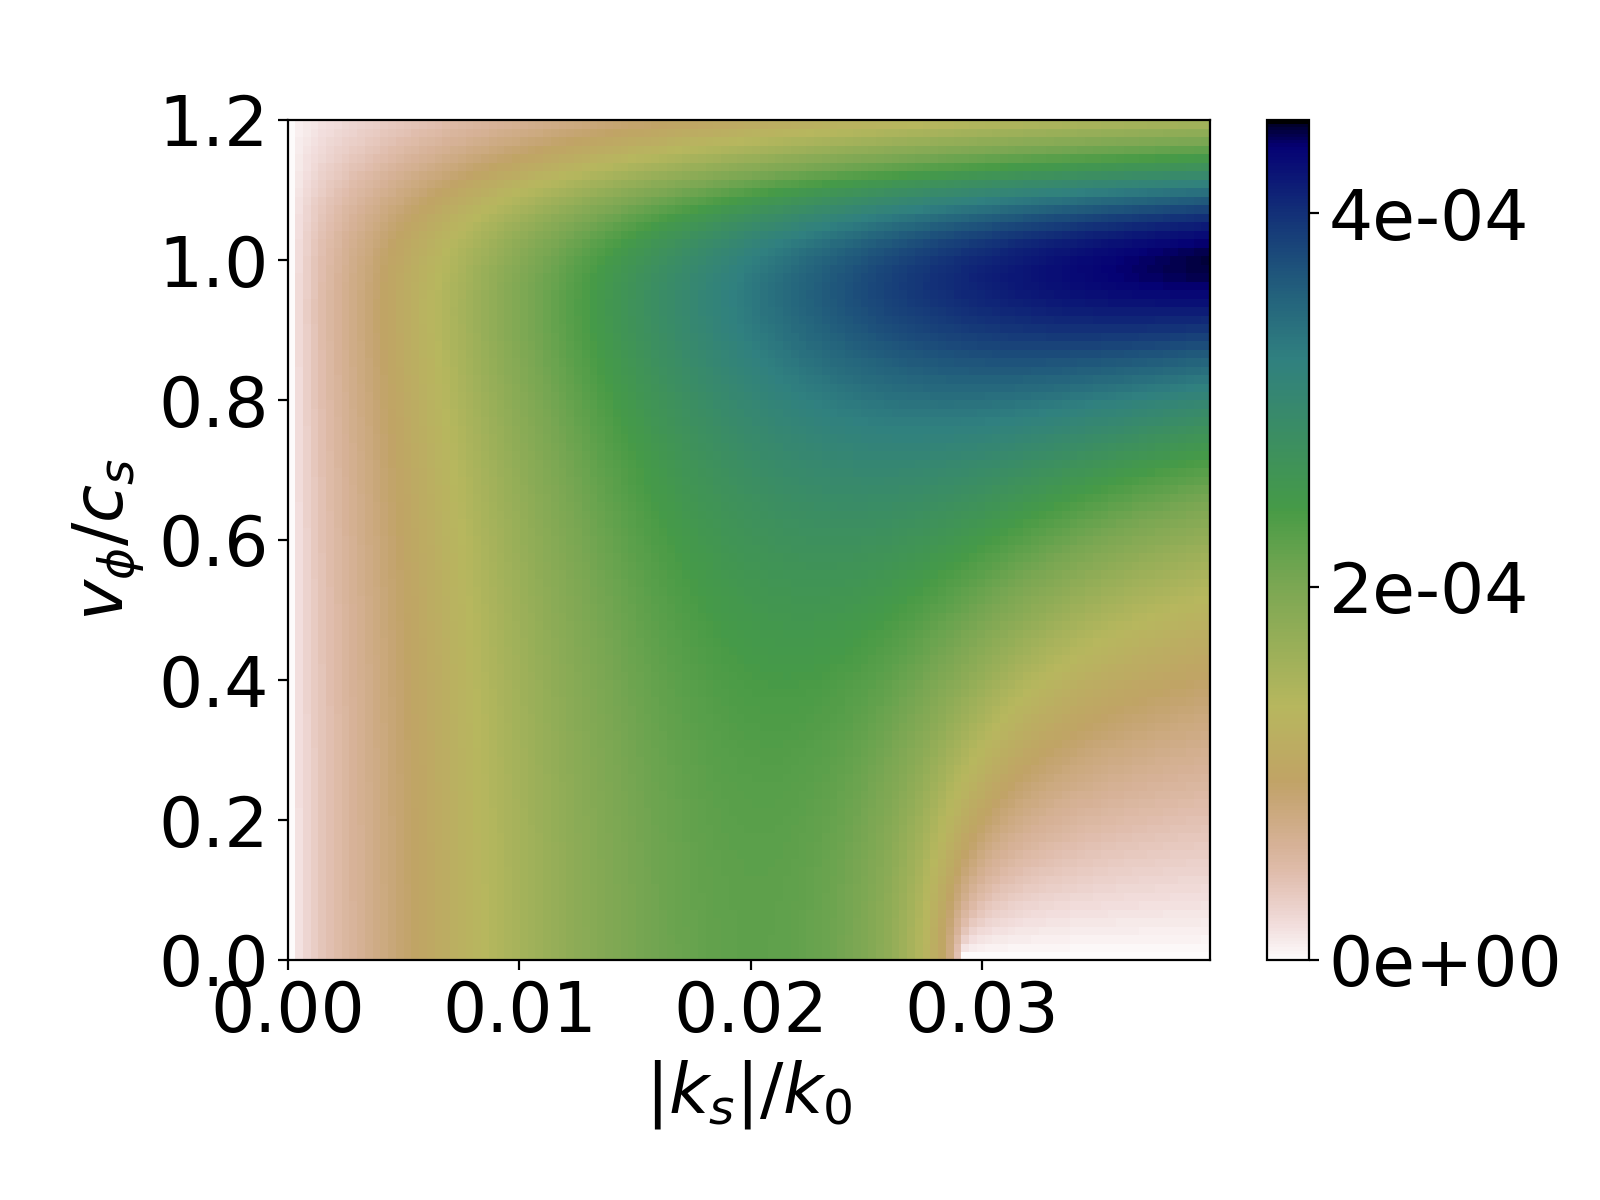
\includegraphics[width=0.24\textwidth]{1a.png}&
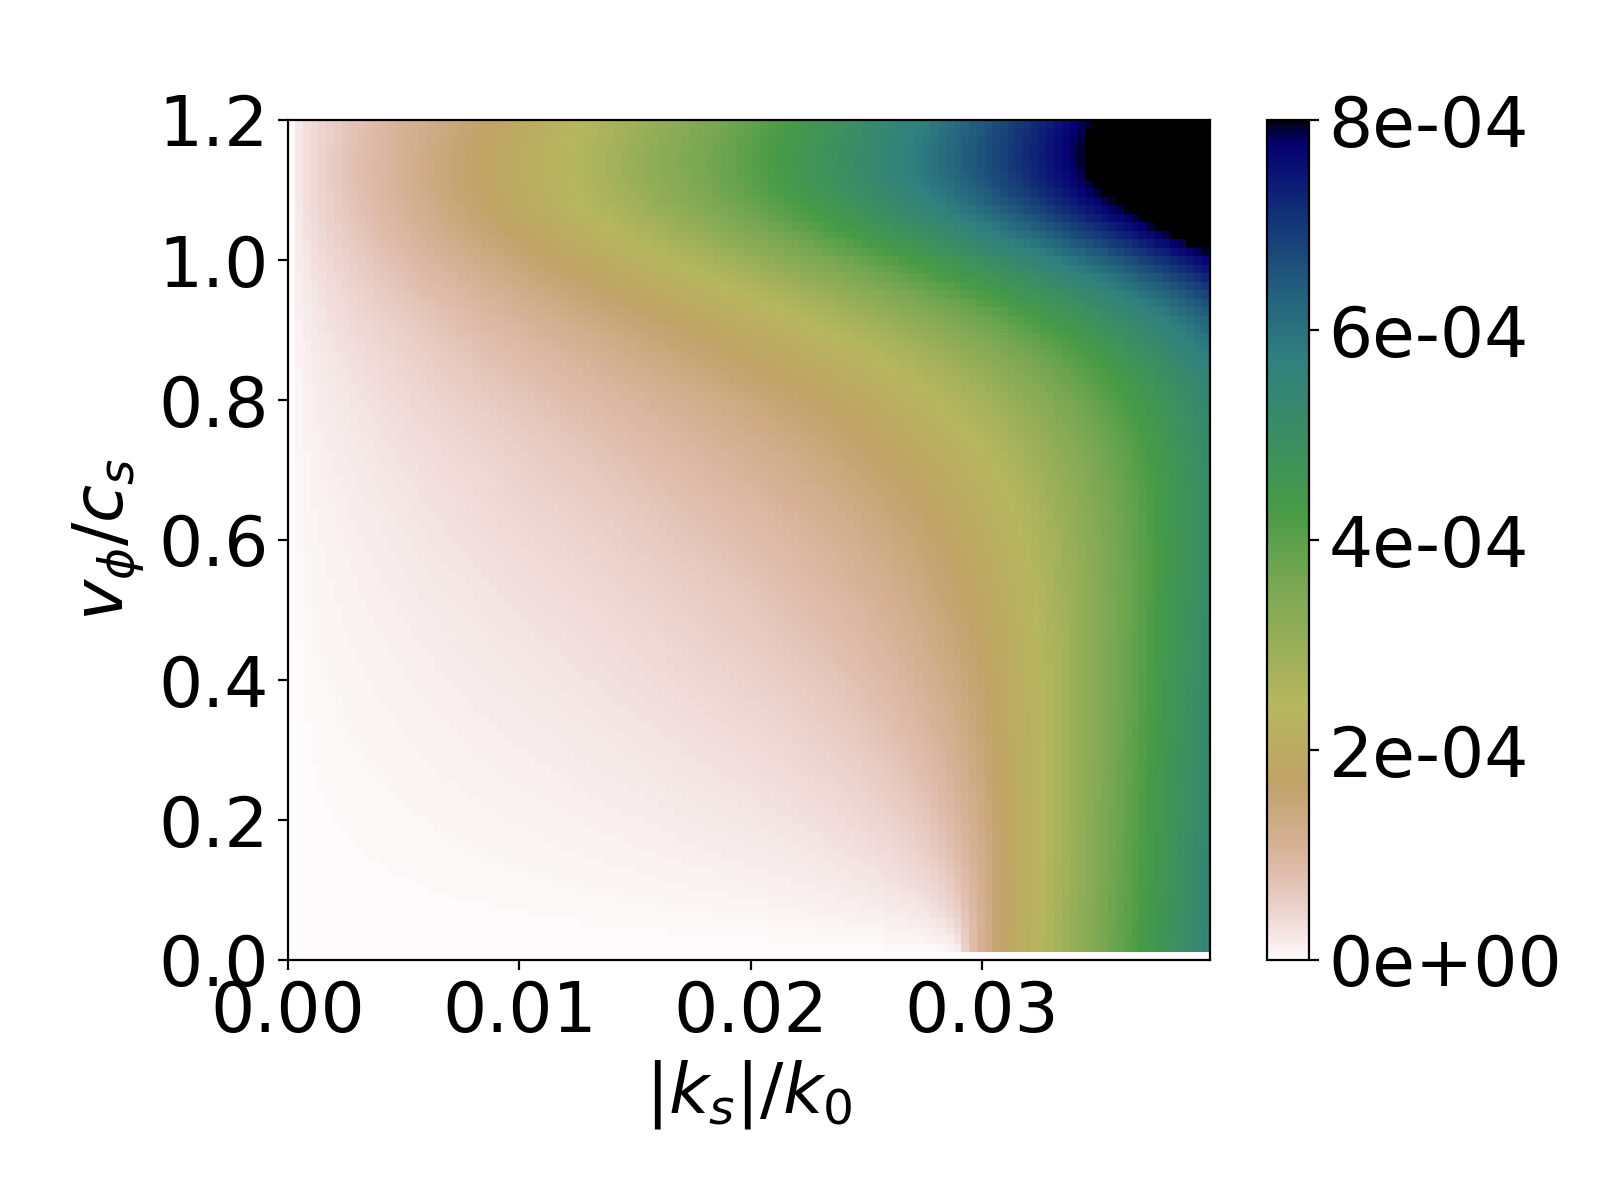
\includegraphics[width=0.24\textwidth]{1b.png}\\
(c) Fluid, $\Gamma/k_0$  &
(d) Fluid, $\Re(k_{sx}/k_0)$  \\
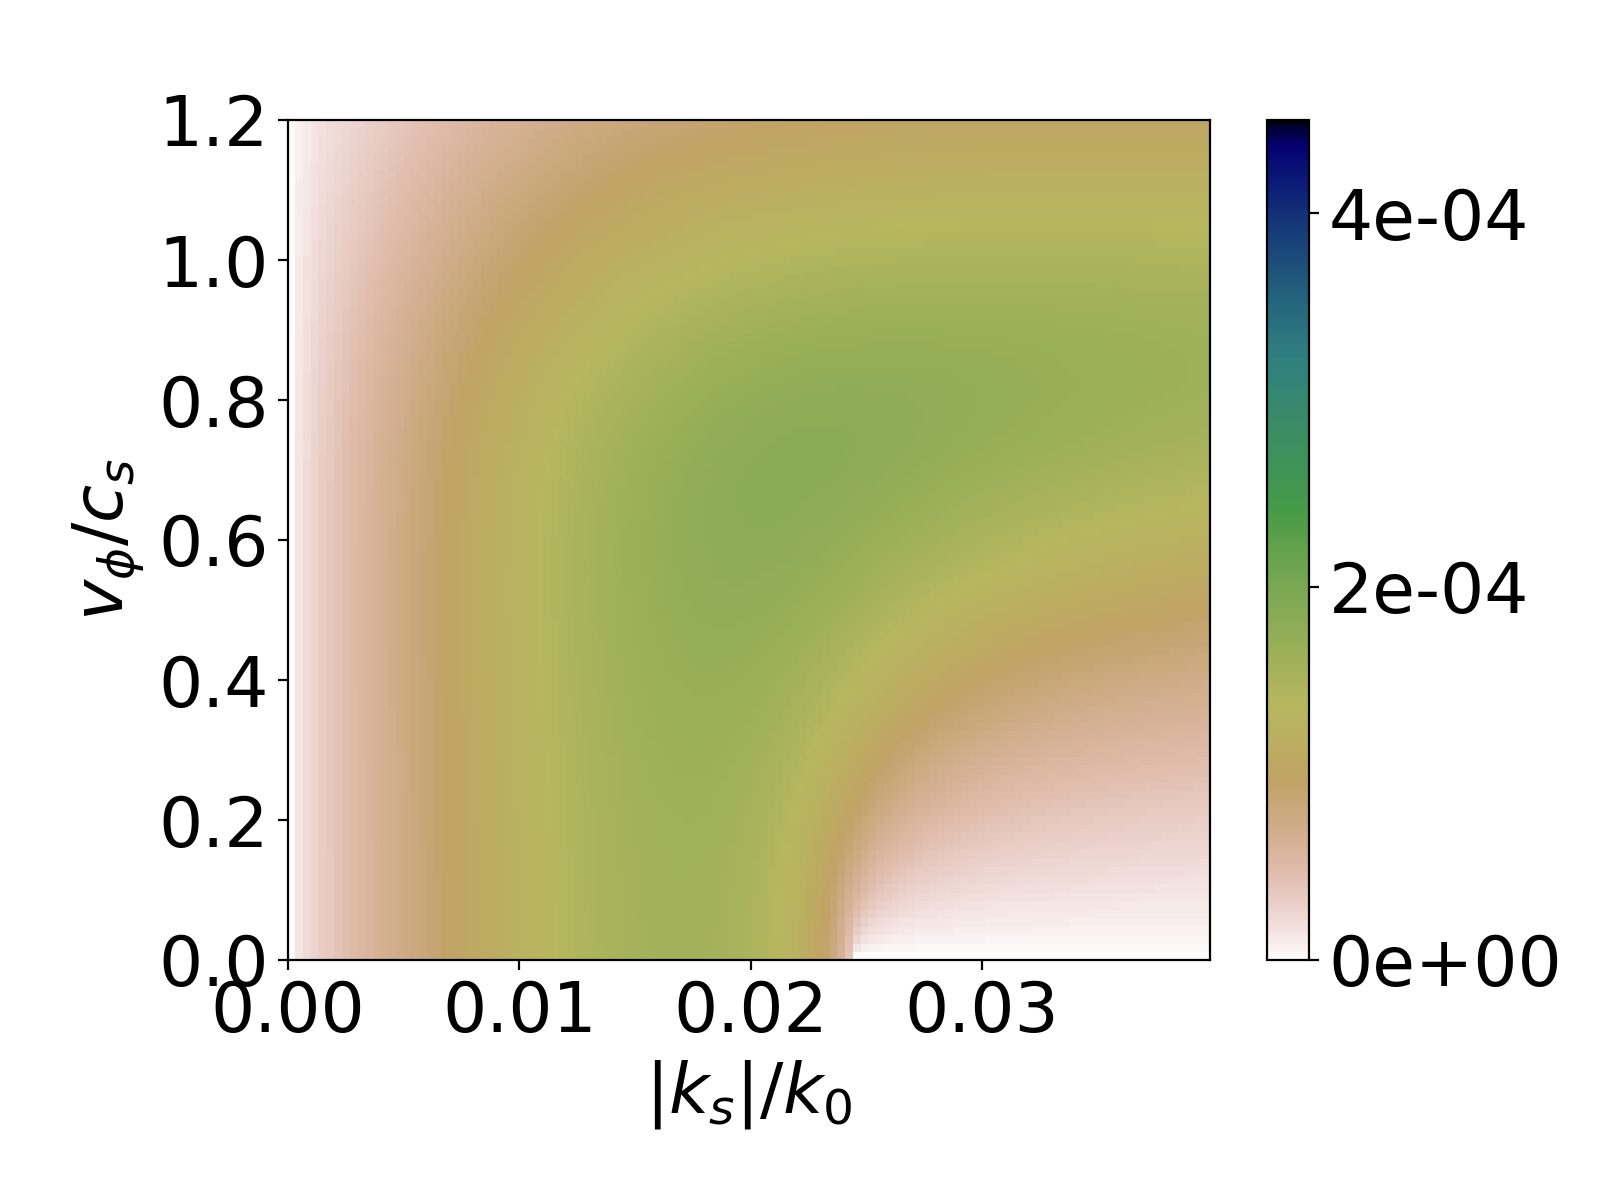
\includegraphics[width=0.24\textwidth]{1c.png}&
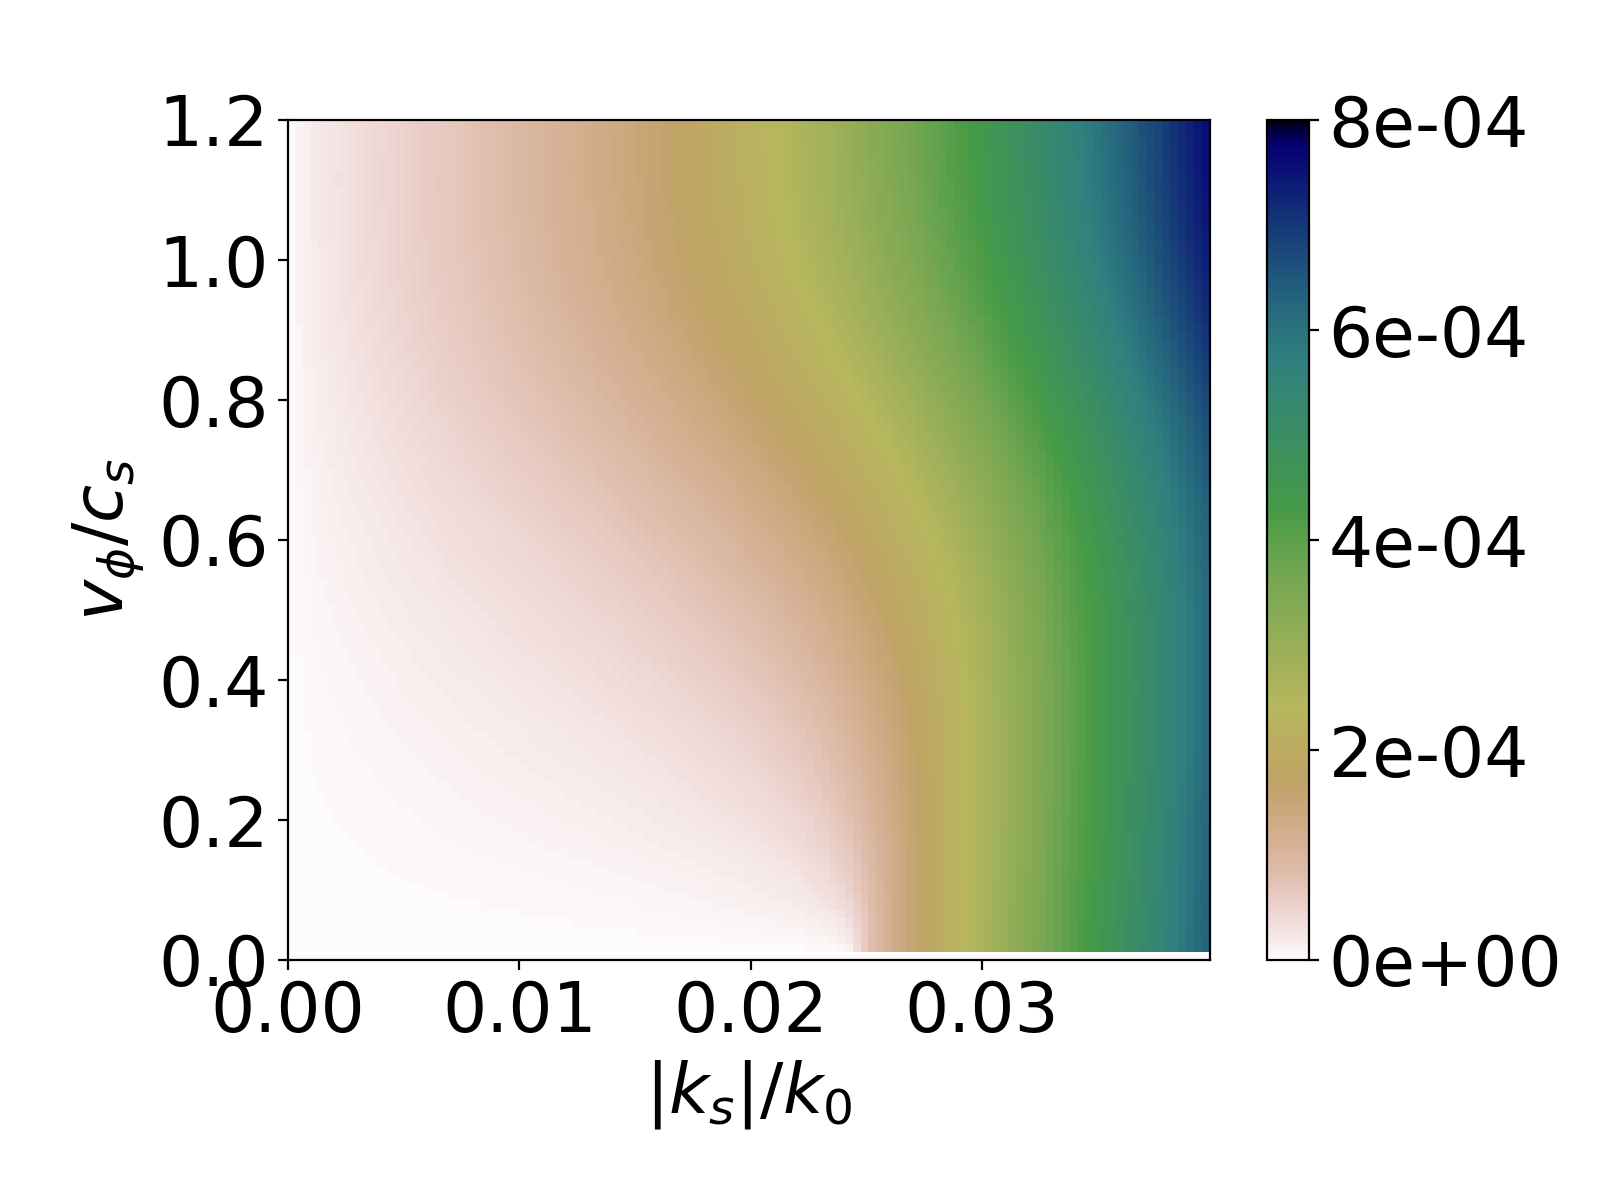
\includegraphics[width=0.24\textwidth]{1d.png}
\end{tabular}
\caption{ \label{fig:dispe}  
Kinetic (a,b) and fluid (c,d) resolution of Eq. \eqref{eq:dispe2poly} for  $I_0 = 6\cdot 10^{14}\, \rm W.cm^{-2}$, $2\pi/k_0=0.35 \,\rm\mu m$, $T_e =1\,\rm  keV$, $ T_i=300\,  \rm eV$ in a H$^+$ and $n_{e0}=0.1n_c$.
 }
\end{figure}
\begin{figure}
\begin{tabular}{cc}
(a) Kinetic, $\Gamma/k_0$ &
(b)  Kinetic, $\Re(k_{sx}/k_0)$ \\
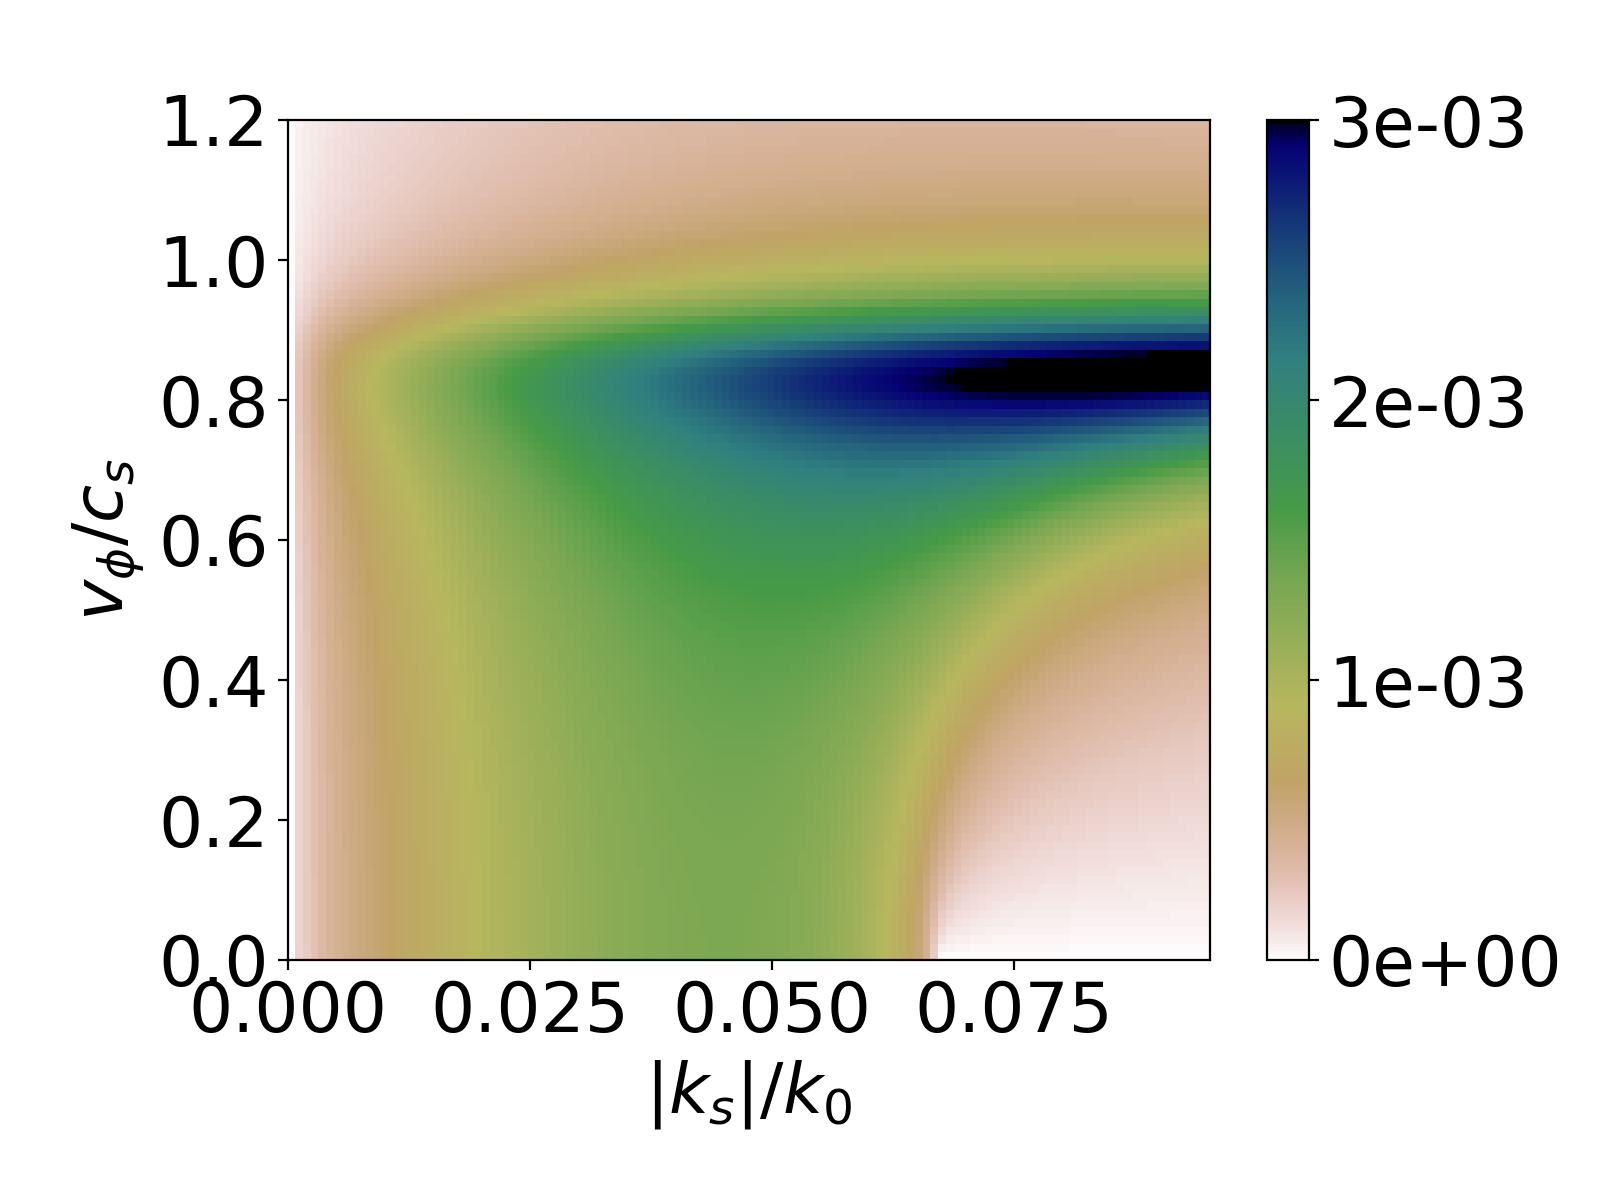
\includegraphics[width=0.24\textwidth]{2a.png}&
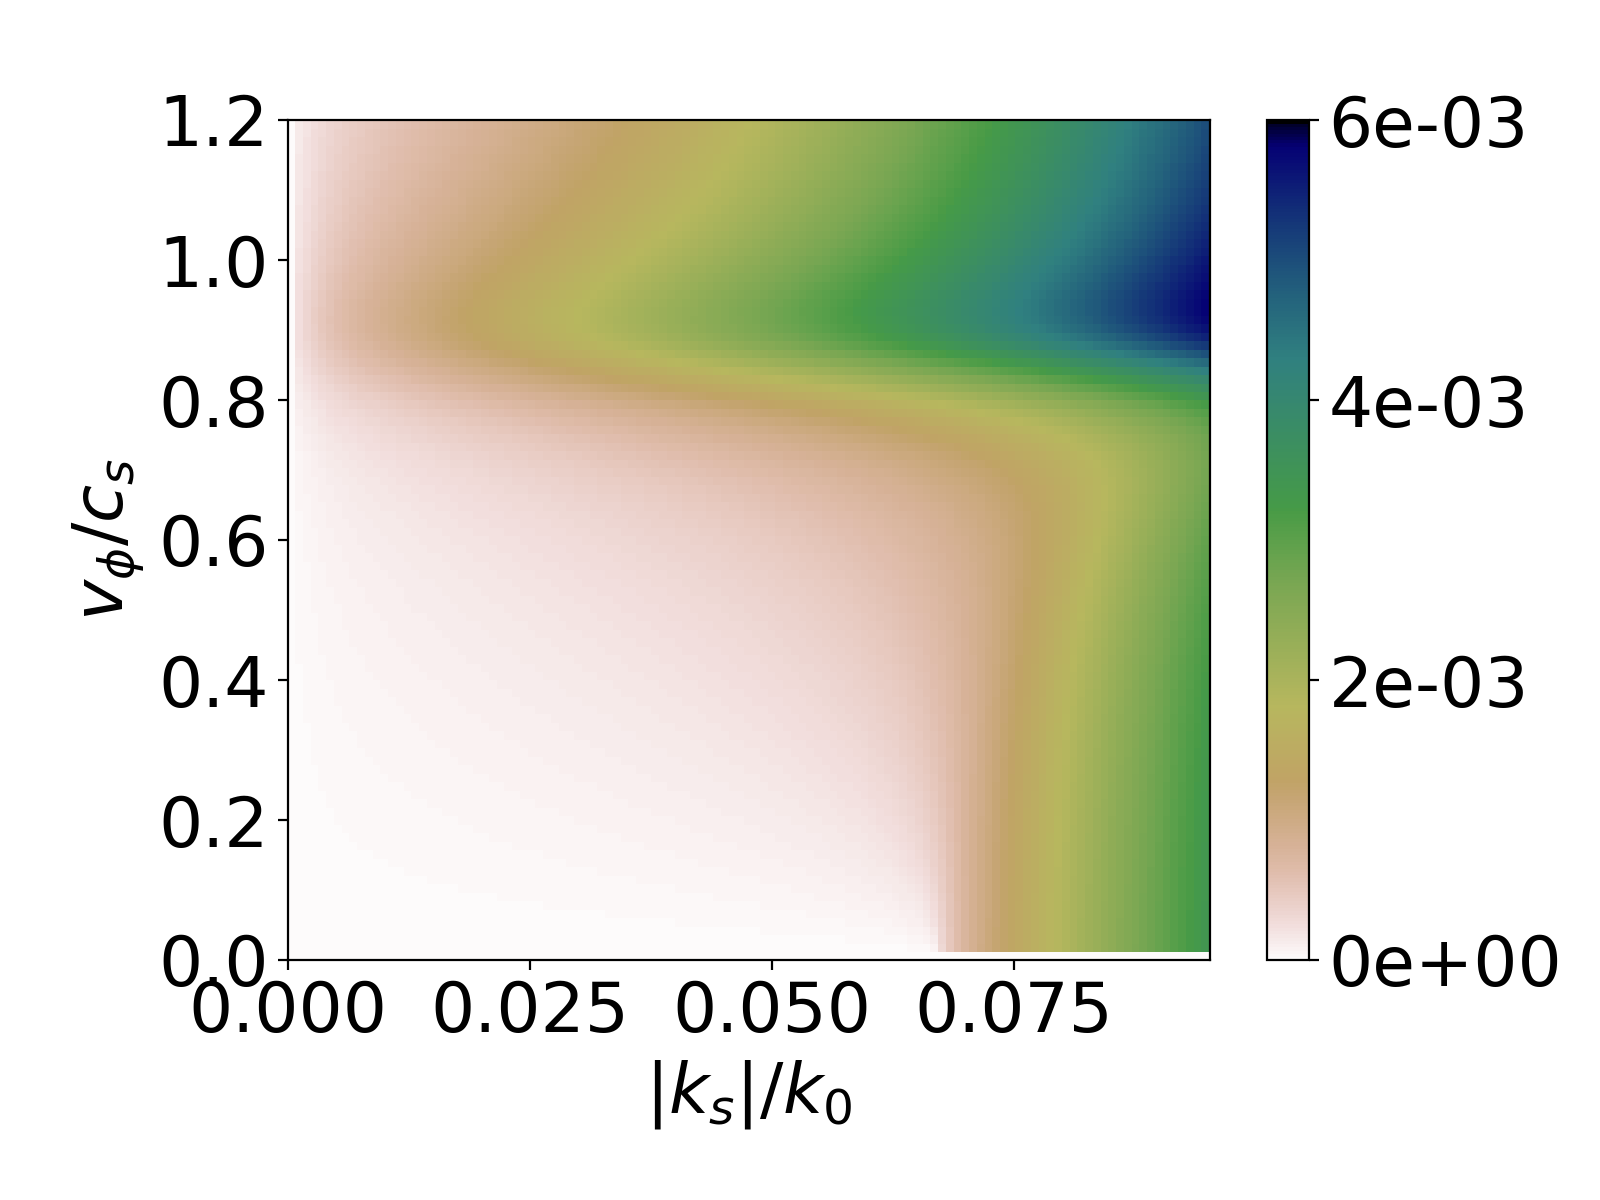
\includegraphics[width=0.24\textwidth]{2b.png}\\
(c) Fluid, $\Gamma/k_0$  &
(d) Fluid, $\Re(k_{sx}/k_0)$  \\
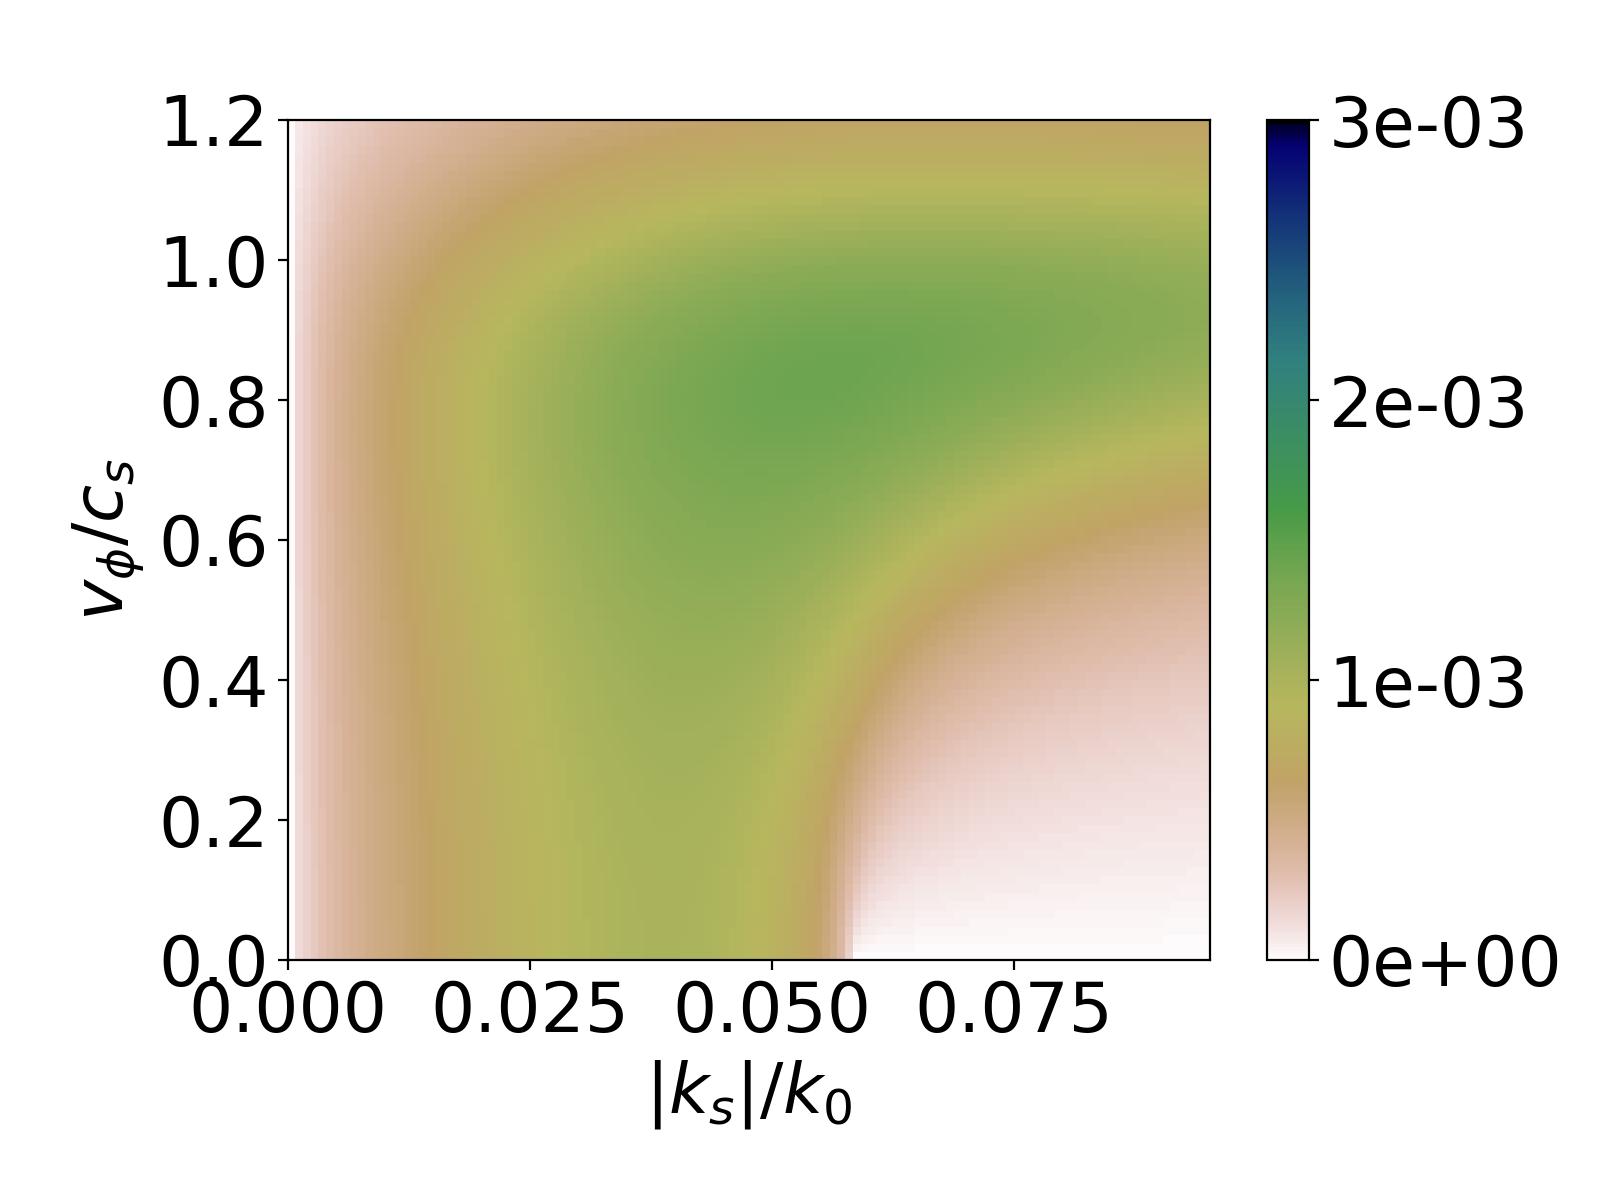
\includegraphics[width=0.24\textwidth]{2c.png}&
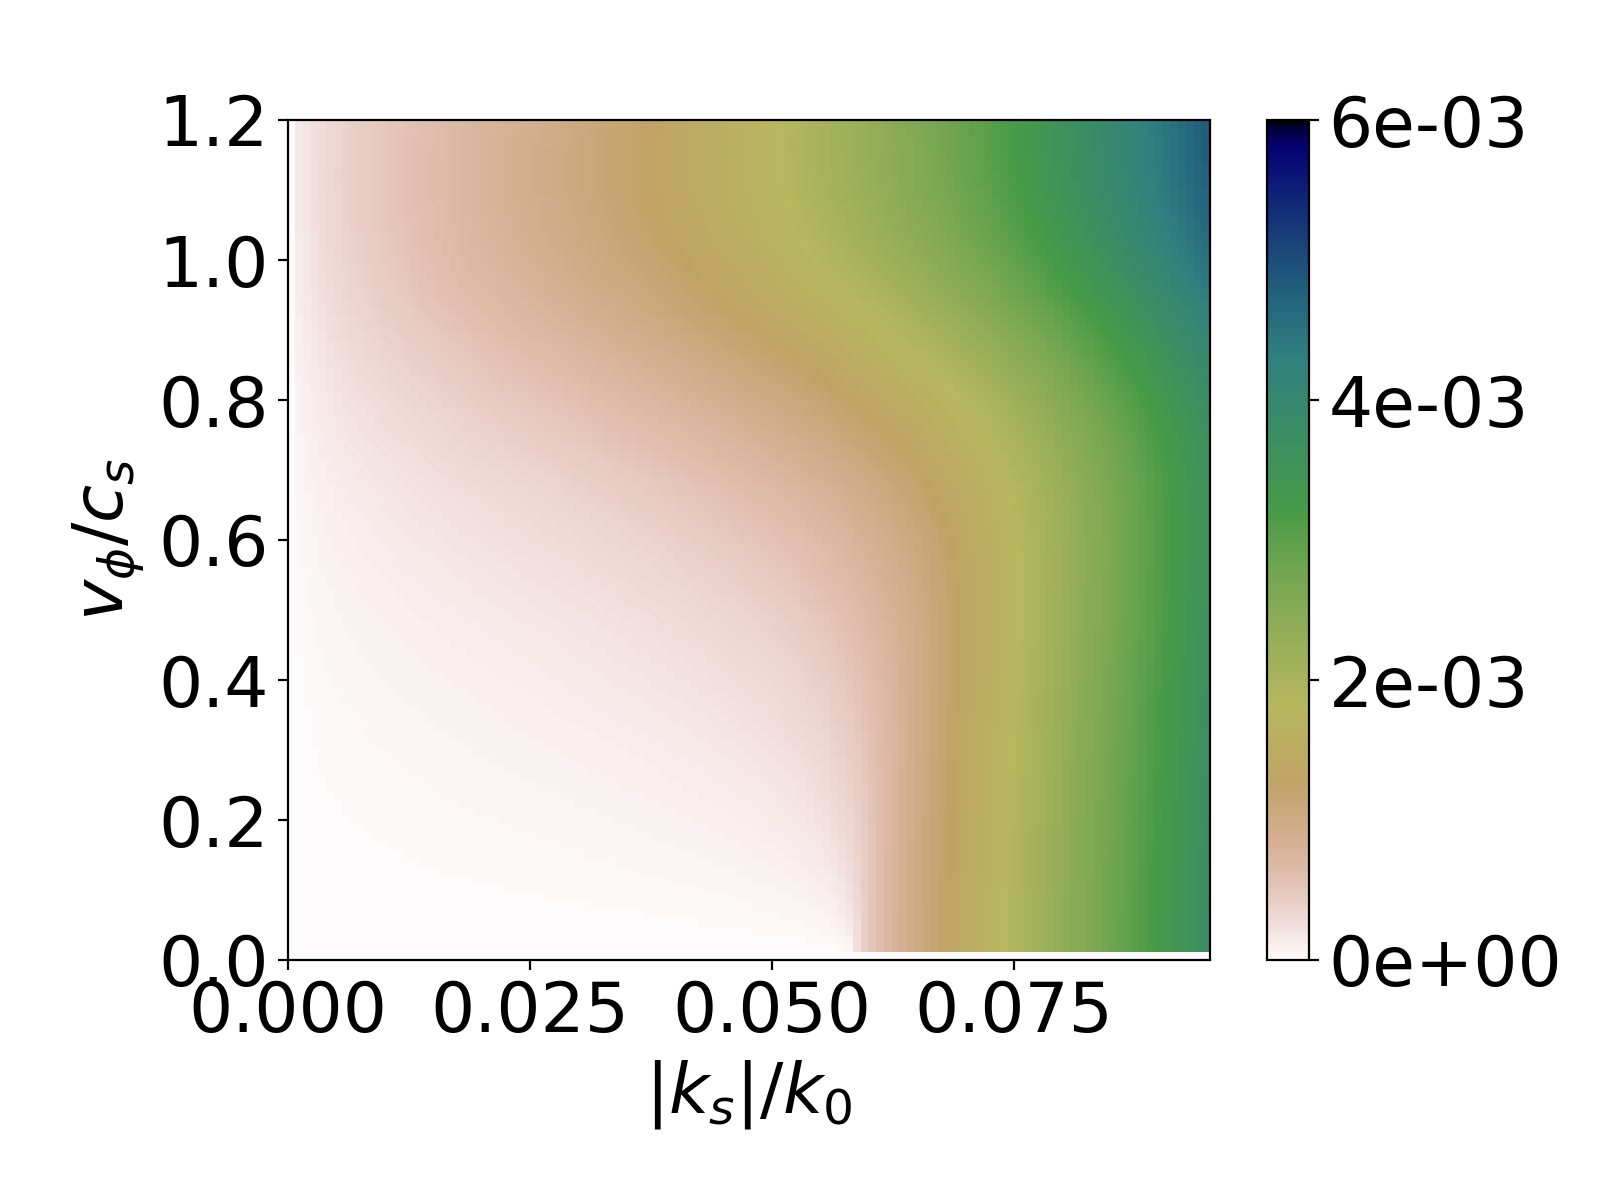
\includegraphics[width=0.24\textwidth]{2d.png}
\end{tabular}
\caption{ \label{fig:dispeCH}  
Kinetic (a,b) and fluid (c,d) resolution of Eq. \eqref{eq:dispe2poly} for  $I_0 = 6\cdot 10^{14}\, \rm W.cm^{-2}$, $2\pi/k_0=0.35 \,\rm\mu m$, for a CH plasma with $n_c=n_H$, $T_e =700\,\rm  eV$, $T_C=T_H =500\,  \rm eV$ and $n_{e0}=0.1n_c$. The value of the non-local correction [Eq. \eqref{eq:nl}], is obtained with the carbon parameters, corresponding to the smallest electron-ion mean-free-path. Use is made of the mean charge number, mean mass number   for calculating the sound speed and normalized Landau damping rate $c_s$ and $\gamma_0$.
 }
\end{figure}
Figures \ref{fig:dispe}(a-d) display  $\Re(k_{sx})$ and the spatial growth rate,  $\Gamma=-\Im(k_{sx})$, combining   the  unstable parts of the two  solutions of Eq. \eqref{eq:dispe2poly} as a function of the phase speed and of the wavevector amplitude, in both the kinetic (a,b) and fluid framework (c,d).
The filamentation limit is recovered at $v_\phi=0$ and care has been taken to verify that, when $T_i\ll Z_iT_e$, both frameworks con\"incide. Moreover, in both calculations, $\Re[k_{sx}(v_\phi=0)]$ is vanishing as expected from the filamentation instability. As $v_\phi$ increases, one starts to enter in the forward Brillouin instability domain which peaks, for the kinetic  mono-ion species case of Fig. \ref{fig:dispe}(a), around $(\vert k_s\vert/k_0, v_\phi/c_s) \simeq(0.03,1)$. Interestingly, only in the kinetic framework  the forward Brillouin spatial maximum  growth dominates the filamentation one, for the plasma parameters addressed here. In the fluid framework however both instability present a close  growth rate of $\sim 1.5\times 10^{-4} k_0$  with much  broader  spectrum than in the kinetic case.

The kinetic calculations allow to consider multiple ion plasmas such as CH as illustrated in Fig. \ref{fig:dispeCH}. In the fluid framework, we are usually constrained to use the averaged-ion approximation, which gives qualitatively similar results than for Fig. \ref{fig:dispe}(c) as a broad spectrum is evidenced with no dominance of the Brillouin versus the filamentation growth. This contrasts with the kinetic calculations of Fig. \ref{fig:dispeCH}(a) where the FSBS is more unstable than the filamentation instability. Moreover the growth is  peaked around $0.8c_s$ (here $c_s$ is calculated on the averaged ion parameters) which is the phase speed of the least-damped acoustic eigenmode, solution of the free-field electrostatic Maxwellian dispersion relation \cite[]{POF_Fried_71,POP_Williams_95}. 

For both Figs. \ref{fig:dispe} and \ref{fig:dispeCH},   from the kinetic framework ensues a  roughly twice lager maximum forward Brillouin growth rate than in the fluid framework,  and comparable results are obtained regarding the filamentation instability. 
The growth of propagating ($\vert v_\phi\vert >0$) ion acoustic wave   is able to  scatter the pump wave and modify its spatial spectrum. As evidenced in Fig. \ref{fig:dispe}(a,d) and \ref{fig:dispeCH}(a,d) we expect a broadening of the plane wave spatial spectrum  resulting in an effective  f-cone   angle  of $k_s/k_0\sim 0.03-0.05$, corresponding to $\sim 2-3^o$.  

The spatial (RPP) or temporal (SSD) of energetic laser pulses is commonly known to restrain the role of deleterious instabilities, such as the laser filamentation, on the propagation of the beam \cite[]{Kato_1984,NatPhys_Glenzer}. Indeed, as shown in this section, the most unstable wavelength, regarding the filamentation or the forward Brillouin instabilities, is of the order of ten   microns (for $\sim$ keV and 10\% critical density plasmas), thus larger than the typical  speckle size   of a few microns   usually used in energetic laser facilities.  
Hence, the plane wave approximation used in obtaining Eq. \eqref{eq:max2} no longer holds and one expects a more stable pump propagation.
Although, extensively studied in the fluid framework by mean of numerical or theoretical tools \cite[]{POP_Schmitt_Afeyan_98,PRL_Myatt_2001,POP_Maximov_2001,Lushnikov_2006,phd-Grech,POP_Grech_2006,PRL_Grech_2009}, to the best of our knowledge, no analytical attempts were made to estimate the spatial growth of the forward Brillouin scattering of an RPP pulse in the kinetic framework. 
We propose in next section to adapt the above analytical plane wave dispersion relations  to tackle this issue.

 \begin{widetext}
\section{Forward scattering of a spatially smoothed laser pulse}
\subsection{Kinetic and fluid dispersion relations}\label{sec:diperpp}
The  beam model adopted here has been introduced in  Refs. \cite[]{POF_Schmitt_88,POF_Rose_93} and presents an electric field which,  at the focal plane depends on time, $t$ and position, $ \mathbf{r}$,
 \begin{align}
E_0(t,\mathbf{r})  = \frac{E_0}{N} \sum_{n,\vert k_{\perp}\vert<k_m }^N  \cos(k_0x - \omega_0t +\mathbf{k}_\perp(n) \cdot \mathbf{r}_\perp +\Phi_{\mathbf{k}_\perp})\, , \label{eq:erpp}
 \end{align}
 where  $N$ is the number of diffracting elements and the phases $\Phi_{\mathbf{k}_\perp}$ are  independent random variables taking the values $0$ or $\pi$ with equal probability.
 For simplicity, we will assume a square phase plate that verifies $k_{\perp}(n) = n2k_m/N$ and  $n$ an integer with $n\in \llbracket - N/2 ,N/2 \rrbracket$ and $k_m = k_0/(2f_\sharp)$. 
 Under these conditions, and for $\langle w\rangle$ representing the statistical average of the random variable $w$,  we note   that,
 \begin{equation}\label{eq:d}
 \langle e^{i\Phi_{k_1}+i\Phi_{k_2}}\rangle=\delta(k_1-k_2) \, .
 \end{equation}

We will now follow the procedure introduced in Sec. \ref{sec:plane} while replacing the plane pump wave by the fields given by Eq. \eqref{eq:erpp}. Hence, we will start by writing the RPP electric field in Fourier space and enveloped around the laser frequency and wavevectors $\omega_0$ and $k_0$, keeping the same notations than in Sec. \ref{sec:plane},
\begin{align}
\mathrm{FT}_{\omega,\mathbf{k} }[E_0(t,\mathbf{r}) ]= \frac{\bar{E_0}}{2N} \sum_{\ k_{\perp} }[ e^{i\Phi_{k_\perp}}\delta(\omega-\omega_0, \mathbf{k}-\mathbf{k}_\perp)    + e^{-i\Phi_{k_\perp}}\delta(\omega+\omega_0, \mathbf{k}+\mathbf{k}_\perp) ]
\, , \label{eq:erppf}
\end{align}
 where $\mathbf{k}_\perp= k_0\hat{\mathbf{x}} +k_\perp \hat{\mathbf{y}}$ and the sum runs over $k_\perp$ for $\vert k_\perp\vert  <k_m$.
 Combined with the perturbed Maxwell equations [Eq. \eqref{eq:max1}], we obtain
 \begin{align}
    (\omega_d^2 - \omega_{pe}^2 -\mathbf{k}_d^2c^2)\delta E(\omega_d,\mathbf{k}_d) = \frac{\omega_0^2}{2N} \bar{E_0} \sum_{\ k_{\perp} }   \left[e^{i\Phi_{k_\perp}}\frac{\delta n_e }{n_c}(\omega_d-\omega_0, \mathbf{k}_d-\mathbf{k}_\perp) +e^{-i\Phi_{k_\perp}}\frac{\delta n_e }{n_c}(\omega_d+\omega_0, \mathbf{k}_d+\mathbf{k}_\perp) \right] \, .\label{eq:maxrpp}
\end{align}
Likewise, the plasma linear response, either kinetic or fluid, involves a convolution product between $E_0(\omega_0,\mathbf{k}_\perp)$ and $\delta E(\omega_d,\mathbf{k}_d)$ which yields,
\begin{align}
   \frac{\delta n_e }{n_{e0}}(\omega_s,\mathbf{k}_s) = -\alpha_{k/f}(v_\phi) \frac{A_k\epsilon_0\bar{E_0}}{Nn_c T_e} \sum_{\ k_{\perp} }     \left[e^{i\Phi_{k_\perp}}\delta E(\omega_s-\omega_0, \mathbf{k}_s-\mathbf{k}_{\perp}) +e^{-i\Phi_{k_\perp}}\delta E(\omega_s+\omega_0, \mathbf{k}_s+\mathbf{k}_{\perp}) \right] \, ,\label{eq:fdrpp} 
\end{align}
When plugging Eq. \eqref{eq:maxrpp} into \eqref{eq:fdrpp}, two sums will appear, noted with two independent index, $k_1$ and $k_2$. Hence, as for the derivation of Eq. \eqref{eq:dispe}, we will neglect the terms in $\delta n_e(\omega_s\pm 2\omega_0)$ that are considered too far from resonance. With $D_\pm(k_{1})= (\omega_s\pm\omega_0)^2 - \omega_{pe}^2 -( k_{sx}\pm k_0) ^2c^2 -( k_{sy}\pm k_{1}) ^2c^2$ and $\mathbf{k}_{1,2}= k_0\hat{\mathbf{x}} +k_{1,2} \hat{\mathbf{y}}$, we obtain
\begin{align}
   \frac{\delta n_e }{n_{e0}}(\omega_s,\mathbf{k}_s) = -\alpha_{k/f}(v_\phi)A_k \frac{\delta n_0}{n_c} \frac{\omega_0^2}{N^2}\sum_{ k_{1} } \sum_{ k_{2} }        \left[ \frac{e^{i\Phi_{k_1}-i\Phi_{k_2}} }{D_-(k_{1})}\frac{\delta n_e }{n_{e0}}(\omega_s,\mathbf{k}_s-\mathbf{k}_{1}+\mathbf{k}_{2}) +\frac{e^{-i\Phi_{k_1}+i\Phi_{k_2}}}{D_+(k_{1})} \frac{\delta n_e }{n_{e0}}(\omega_s,\mathbf{k}_s+\mathbf{k}_{1}-\mathbf{k}_{2}) \right] \, ,\label{eq:fddrpp} 
\end{align}
 \end{widetext}
 
 \begin{figure}
\begin{tabular}{cc}
(a) Kinetic, $\Gamma/k_0$ &
(b)  Kinetic, $\Re(k_{sx}/k_0)$ \\
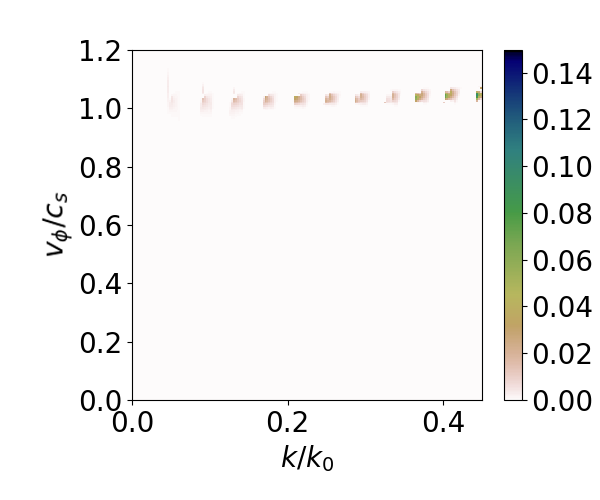
\includegraphics[width=0.24\textwidth]{gkH300eV.png}&
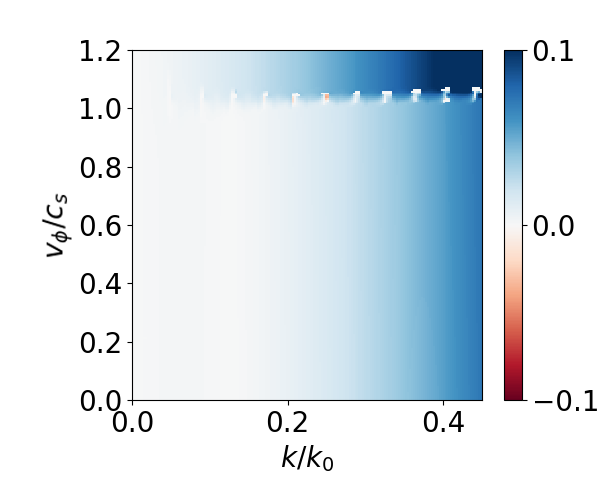
\includegraphics[width=0.24\textwidth]{kkH300eV.png}\\
(c) Fluid, $\Gamma/k_0$  &
(d) Fluid, $\Re(k_{sx}/k_0)$  \\
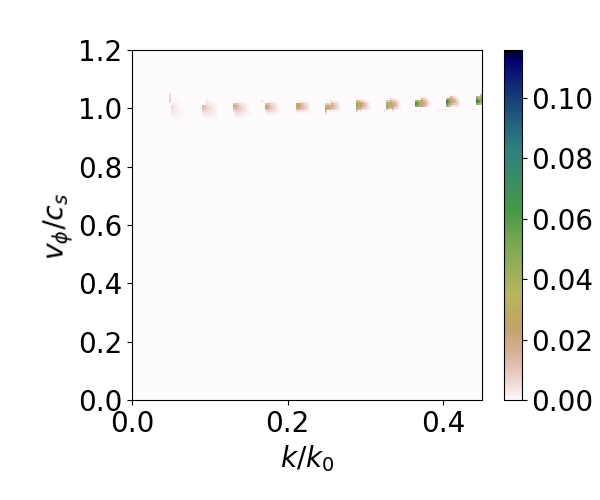
\includegraphics[width=0.24\textwidth]{gfH300eV.png}&
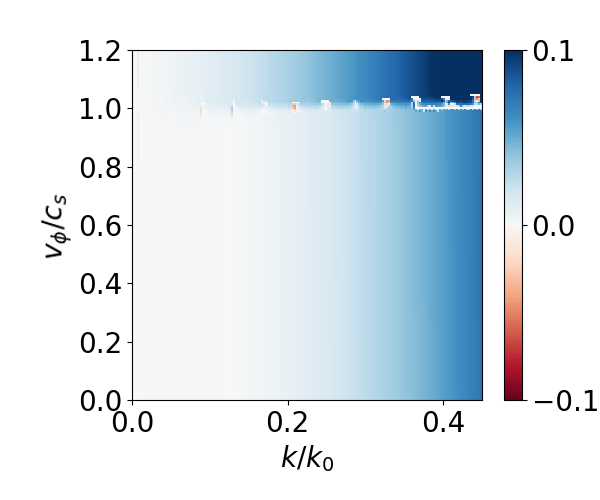
\includegraphics[width=0.24\textwidth]{kfH300eV.png}
\end{tabular}
\caption{ \label{fig:disperpp}  
Kinetic (a,b) and fluid (c,d) resolution of Eq. \eqref{eq:dispe2polyrpp} for  the same parameters than in Fig. \ref{fig:dispe} but with an RPP beam given by Eq. \eqref{eq:erpp} with $f_\sharp=8$. 
 }
\end{figure}
\begin{figure}
\begin{tabular}{cc}
(a) Kinetic, $\Gamma/k_0$ &
(b)  Kinetic, $\Re(k_{sx}/k_0)$ \\
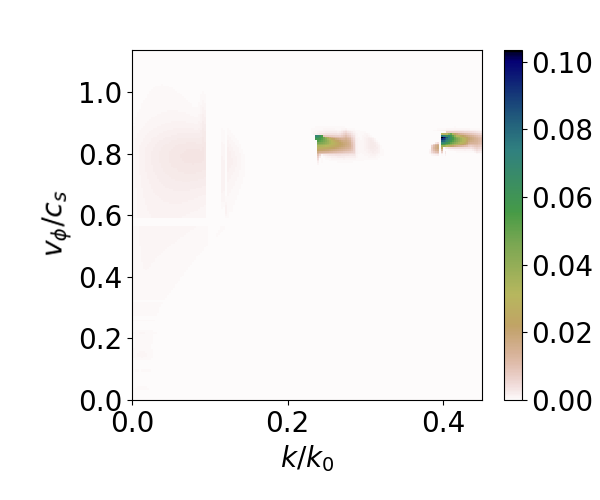
\includegraphics[width=0.24\textwidth]{gkCH300eV.png}&
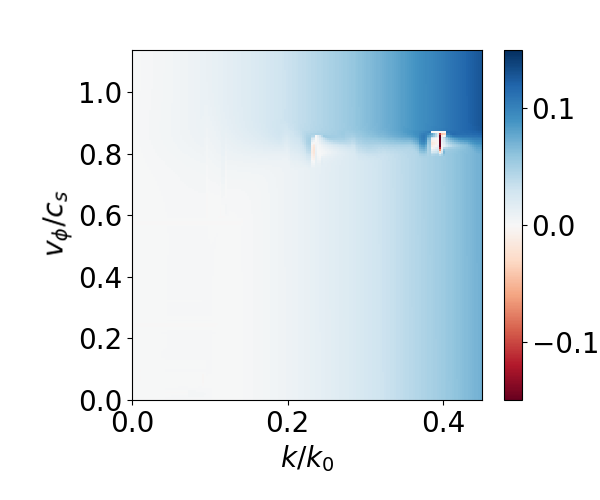
\includegraphics[width=0.24\textwidth]{kkCH300eV.png}\\
(c) Fluid, $\Gamma/k_0$  &
(d) Fluid, $\Re(k_{sx}/k_0)$  \\
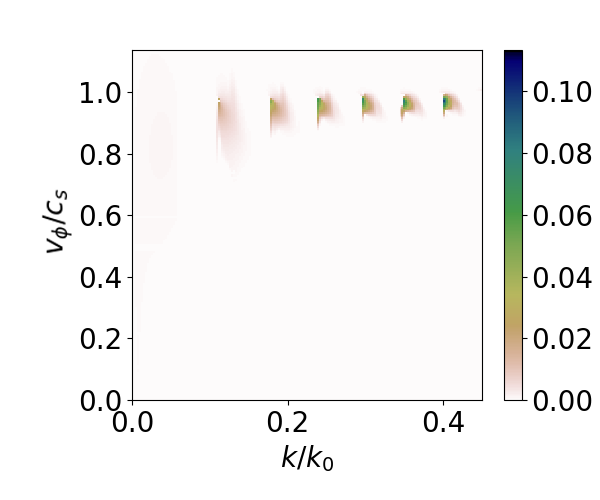
\includegraphics[width=0.24\textwidth]{gfCH300eV.png}&
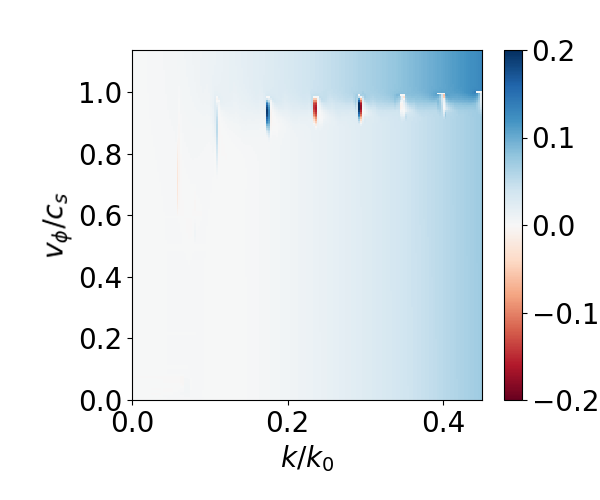
\includegraphics[width=0.24\textwidth]{kfCH300eV.png}
\end{tabular}
\centering{(e) lineout at $v_\phi=0$}\\
\centering{
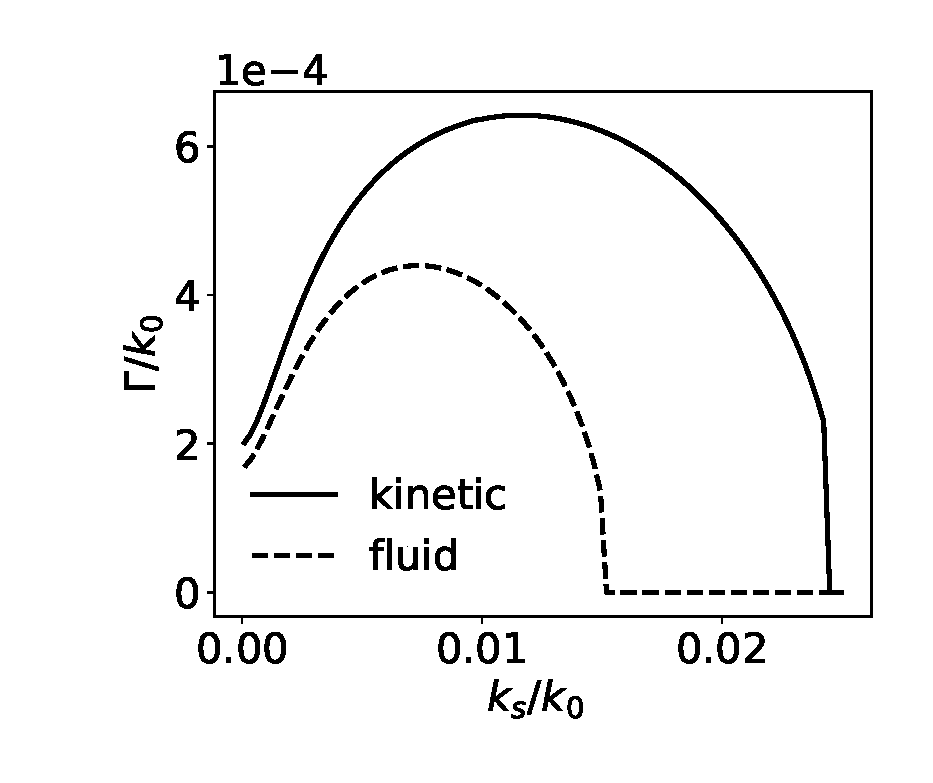
\includegraphics[width=0.24\textwidth]{filamCH.eps}
}
\caption{ \label{fig:dispeCHrpp}  
Kinetic (a,b) and fluid (c,d) resolution of Eq. \eqref{eq:dispe2polyrpp} for  the same parameters than in Fig. \ref{fig:dispeCH} but with an RPP beam given by Eq. \eqref{eq:erpp} with $f_\sharp=8$.  The value of the non-local correction [Eq. \eqref{eq:nl}], is obtained with the carbon parameters, corresponding to the smallest electron-ion mean-free-path. Use is made of the mean charge number, mean mass number   for calculating the sound speed and normalized Landau damping rate $c_s$ and $\gamma_0$.
Panel (e) corresponds to lineouts at $v_\phi=0$ of (a) and (c). 
 }
\end{figure}
In order to finalize the RPP dispersion relation, we will proceed to a statistical averaged using Eq. \eqref{eq:d}. On the right-hand-side, appears $\langle\exp(-i\Phi_{k_1}+i\Phi_{k_2})\delta n_e \rangle$ which can be recast as
\begin{equation}
\langle\exp(-i\Phi_{k_1}+i\Phi_{k_2})\delta n_e \rangle= \langle\exp(-i\Phi_{k_1}+i\Phi_{k_2}) \rangle\langle\delta n_e \rangle + \mathcal{C}\, , \label{eq:mthcalc}
\end{equation}
where $\mathcal{C}$ is the correlations   between  \mbox{$\exp(-i\Phi_{k_1}+i\Phi_{k_2})$} and $\delta n_e$. The combination of Eq. \eqref{eq:fddrpp} with \eqref{eq:mthcalc} shows that $\mathcal{C}\propto \delta n_0/n_c$ and therefore, to leading order in $\delta n_0/n_c$, $\mathcal{C}$ may  be neglected when  averaging   Eq. \eqref{eq:fddrpp} giving
\begin{align}
  1= -\alpha_{k/f}(v_\phi)A_k \frac{\delta n_0}{n_c} \frac{\omega_0^2}{N}\sum_{ k_{1} }        \left[ \frac{1 }{D_-(k_{1})} +\frac{1}{D_+(k_{1})} \right] \, .\label{eq:disperpp} 
\end{align}
Provided the phase plate has a sufficient number of elements (\emph{i.e.} $N$ is large enough), we shall replace the discrete sum by a continuous one. To leading order 
in  $\omega_s\ll\omega_0$, 
\begin{equation}\label{eq:dpmk1}
D_\pm(k_1) \simeq -\mathbf{k}_s^2c^2\pm 2(\omega_s\omega_0 - k_{sx}k_0 c^2-k_{sy} k_1 c^2) \, , 
\end{equation} 
so that,
\begin{align}
 \frac{1}{N} \sum_{ k_{1} }  \frac{1 }{D_\pm(k_{1})}  \simeq \frac{1}{2k_m} \int_{ -k_m }^{ k_m }       \frac{dk_1 }{D_\pm(k_{1})}  \, , \nonumber\\
 \simeq \frac{\mp1}{4k_mk_{sy}c^2} \ln\left[
 \frac{ -\mathbf{k}_s^2c^2\pm 2(\omega_s\omega_0 - k_{sx}k_0 c^2-k_{sy} k_m c^2)}{ -\mathbf{k}_s^2c^2\pm 2(\omega_s\omega_0 - k_{sx}k_0 c^2+k_{sy} k_m c^2)} \right] \, .\label{eq:sumint} 
\end{align}
The combination with Eq. \eqref{eq:disperpp} yields
\begin{align}
 \frac{-4k_mk_{sy}c^2}{\alpha_{k/f}(v_\phi)A_k \omega_0^2\delta n_0/n_c  } \nonumber\\
 \simeq  \ln\left[
 \frac{ (\mathbf{k}_s^2c^2-2k_{sy} k_m c^2)^2 -4(\omega_s\omega_0 - k_{sx}k_0 c^2)^2}{ (\mathbf{k}_s^2c^2+2k_{sy} k_m c^2)^2 -4(\omega_s\omega_0 - k_{sx}k_0 c^2)^2} \right] \, .\label{eq:disperpp2} 
\end{align}
In order to express the complex $k_{sx}$ as a function of the reals $v_\phi=\omega_s/\vert \mathbf{k}_s\vert $ and $\vert \mathbf{k}_s\vert $, we may assume  $\vert k_{sy} \vert  \simeq \vert \mathbf{k}_s\vert$ (provided  $\vert k_{sx}\vert \ll \vert \mathbf{k}_s\vert$), and divide both numerator and denominator of the logarithm argument by $k_0^2\vert \mathbf{k}_s^2\vert c^4$, which yields the following second order polynomial equation in $u =  k_{sx}/\vert \mathbf{k}_s\vert$,
\begin{align}
u^2 -2\frac{v_\phi}{\eta c}u +\frac{v_\phi^2}{\eta^2 c^2}-\frac{1}{4}A =0 
\, , \label{eq:dispe2polyrpp} \\
A= \frac{1}{1-B}\left[ \left(\frac{\vert k_{s}\vert}{k_0}-\frac{1}{f_\sharp}\right)^2-\left(\frac{\vert k_{s}\vert}{k_0}+\frac{1}{f_\sharp}\right)^2B  \right]\, , \label{eq:dispe2polyrpp1}  \\ 
B =\exp\left(\dfrac{-4k_m \vert k_{s}\vert c^2}{\alpha_{k/f}(v_\phi)A_k \omega_0^2\delta n_0/n_c  }\right)\, .
\label{eq:dispe2polyrpp2} 
\end{align}
The last term of the left hand side of  Eqs. \eqref{eq:dispe2poly} and \eqref{eq:dispe2polyrpp} holds the only difference between plane wave and RPP dispersion relations. 
As expected,  Eqs.   \eqref{eq:dispe2poly} and     \eqref{eq:dispe2polyrpp} coincide when  a Taylor expansion of $A$ [Eq. \eqref{eq:dispe2polyrpp1}] to first order  in $1/f_\sharp$ is made, \emph{i.e.} for a vanishing  RPP beam spectral width, $2k_m=k_0/f_\sharp$.
Moreover, care has been taken to verify that the solution of the RPP dispersion relations with  $f_\sharp \ge 50$ yields  very similar results than the solution of Eq. \eqref{eq:dispe2poly}.

The spatial growth rate and wavevector  longitudinal component of the RPP forward scatter are illustrated in  
Figs. \ref{fig:disperpp} and \ref{fig:dispeCHrpp} with identical plasma and laser parameters than Figs.  \ref{fig:dispe} and \ref{fig:dispeCH}, respectively and  with $f_\sharp=8$. 
%They have been obtained by retaining the growing part of both solutions of Eq. \eqref{eq:dispe2polyrpp}.
%
Finally, the assumption made in deriving Eq. \eqref{eq:dispe2polyrpp} ($\vert k_{sx}\vert \ll \vert \mathbf{k}_s\vert$) is, for the parameters of interest here, scarcely  verified [see Figs. \ref{fig:disperpp}(b,d)  \ref{fig:dispeCHrpp}(b,d) for which  $\mathrm{max}(\vert k_{sx}\vert/ \vert \mathbf{k}_s\vert)\sim 0.2$]. Hence, the dispersion relation solutions presented here stems from a non linear algebraic solver applied on Eq. \eqref{eq:disperpp2} (or using a dichotomous algorithm applied at fixed  $v_\phi$ and starting from low values of $\vert \mathbf{k}_s\vert$ ) and  seeded by the approximated solution of Eq. \eqref{eq:dispe2polyrpp} yielding convergence toward the exact solution. 

Hence, regarding the FSBS, no simple stability criterion could be extracted from our dispersion relation such as the one proposed in Refs. \cite[]{Lushnikov_2006,phd-Grech,PRL_Grech_2009}.
This also implies that, in contrast with the plane wave case, the FSBS growing of a RPP beam induces acoustic fluctuations which propagating axis may  have a finite $x$ component, thus   complicating  the subsequent comparison with numerical results.

\subsection{Filamentation of a spatially smoothed beam}\label{sec:filam}
Regarding the H$^+$-plasma case (Fig. \ref{fig:disperpp}), one striking (but expected, see Refs. \cite[]{NatPhys_Glenzer,PRL_Sarri_2011}) difference with the plane wave case  (Fig. \ref{fig:dispe}) is that the propagation of the smoothed beam seems to be stable regarding the filamentation instability, at $v_\phi=0$ [in that case, Eq. \eqref{eq:dispe2polyrpp} simplifies to $u^2=A/4$].
Physically, the speckle typical size, $f_\sharp\lambda_0$, remains smaller than the most unstable filamentation wavelength [$\sim 10 \,\rm\mu m$ in Fig . \ref{fig:dispe}(a)] thus preventing the transverse standing electrostatic wave to grow. The artificial increase of $f_\sharp$ in excess of $\sim 25$, \emph{i.e.} when the speckle size starts to be comparable to the plane wave most unstable wavelength,  yields a finite value of the filamentation spatial growth rate. 
For more moderate  $f_\sharp$-numbers, the propagation of a laser may  also remains filamentation-unstable, despite the use of random phase plates,  in  the case of a multi-ion species plasmas such as in Fig.   \ref{fig:dispeCHrpp}. Although less filamentation unstable than in the plane wave case [see Figs. \ref{fig:dispe}(a,c) and \ref{fig:dispeCH}(a,c)], in both the RPP fluid and kinetic frameworks, a finite peak growth rate of $\sim 4\times 10^{-4}k_0 $ and $\sim 6\times 10^{-4}k_0 $ respectively  are observed around $\vert k_s\vert \sim  10^{-2}k_0$ [see Fig. \ref{fig:dispeCHrpp}(e)].
Hence, the estimated  gain of $\sim 7-10$   for a millimeter of propagation (with a wavelength of $\sim 35 \,\rm \mu m$) indicates that keV-range plasmas may produce significant RPP-laser filamentation, at least in the multi ion species case.
Interestingly, we note that  for our parameters, the fluid average-ion calculations yields a growth maximum   $\sim 30\%$ below the kinetic ones. Hence, a qualitative-only  predictability of hydrodynamic codes regarding the filamentation instability is to be expected in the multi-ion species case.

\subsection{Comparison with proton radiographs of a RPP pulse propagating in a helium gaz jet}\label{sec:xp}
\begin{figure}
(a) Setup \\
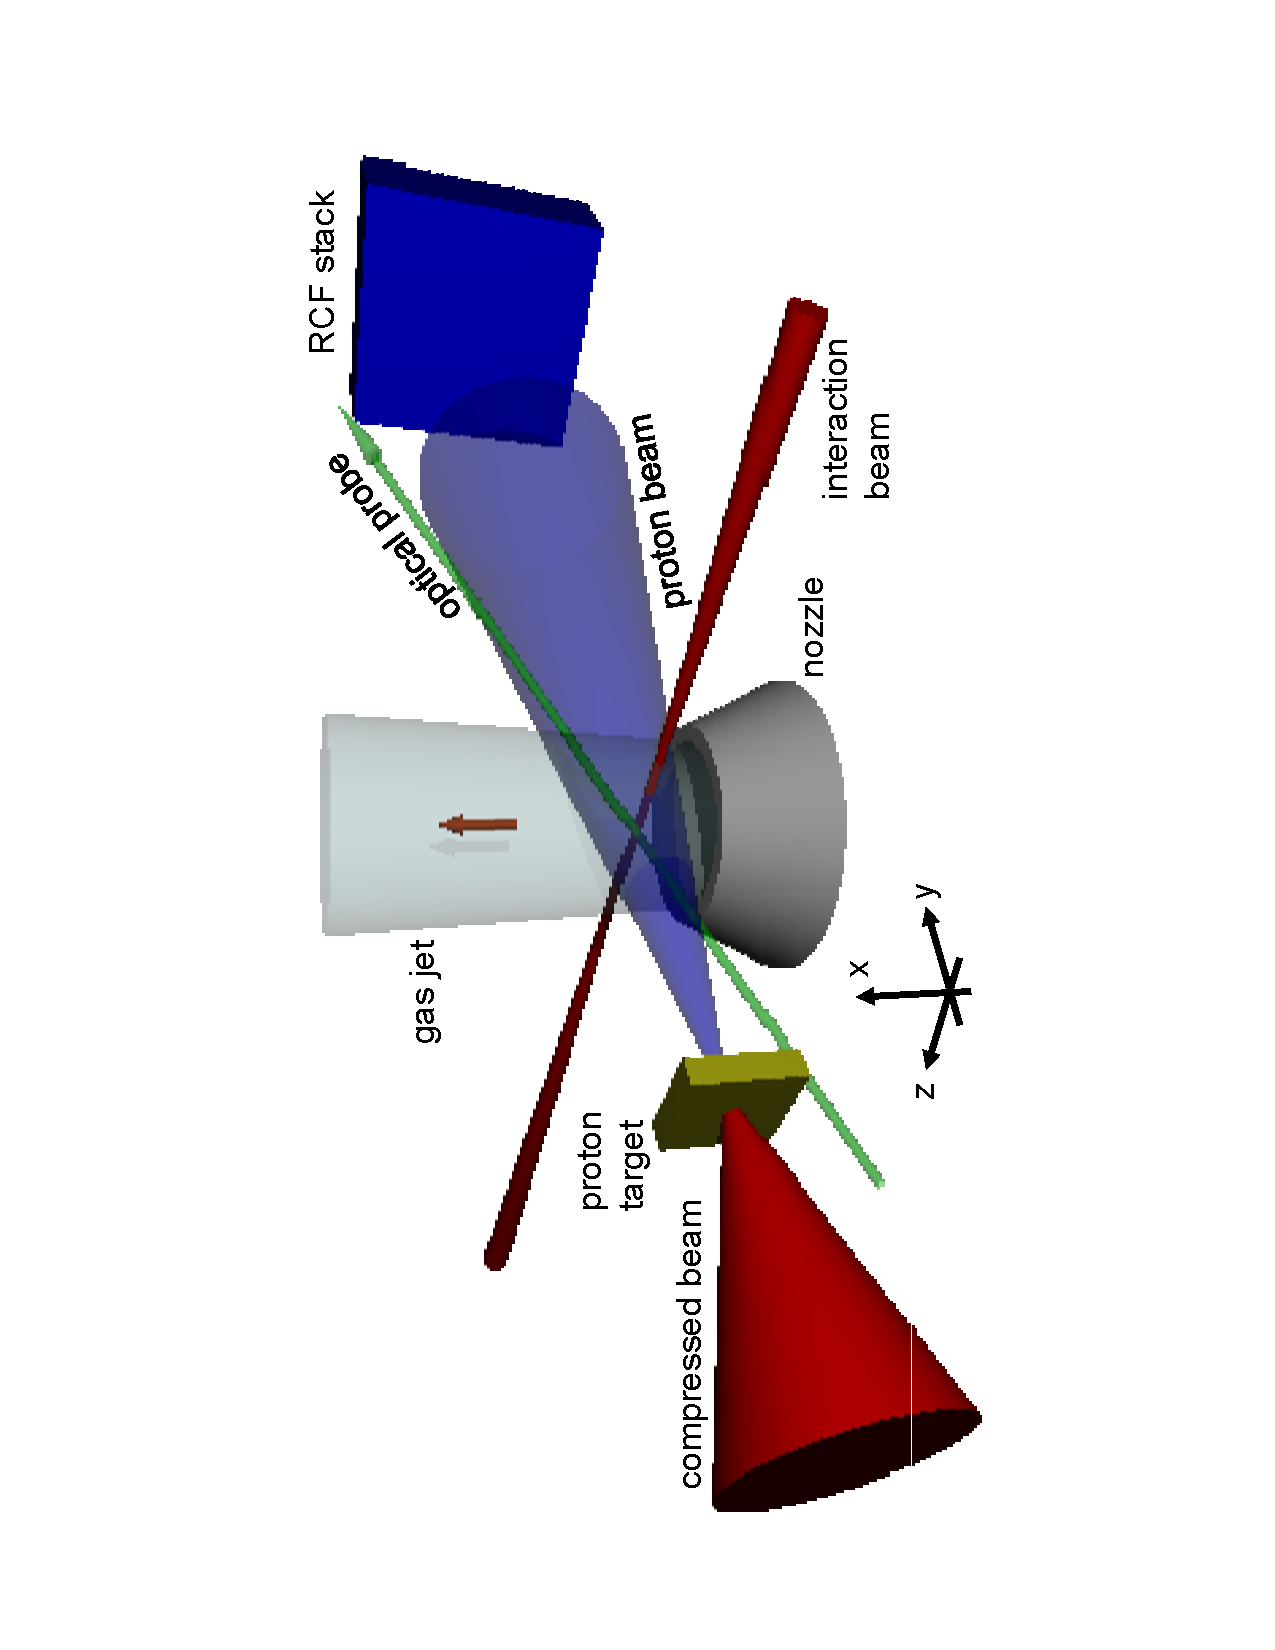
\includegraphics[width=0.4\textwidth,angle=-90]{set_up.pdf}\\
(b) Experimental RCF \\
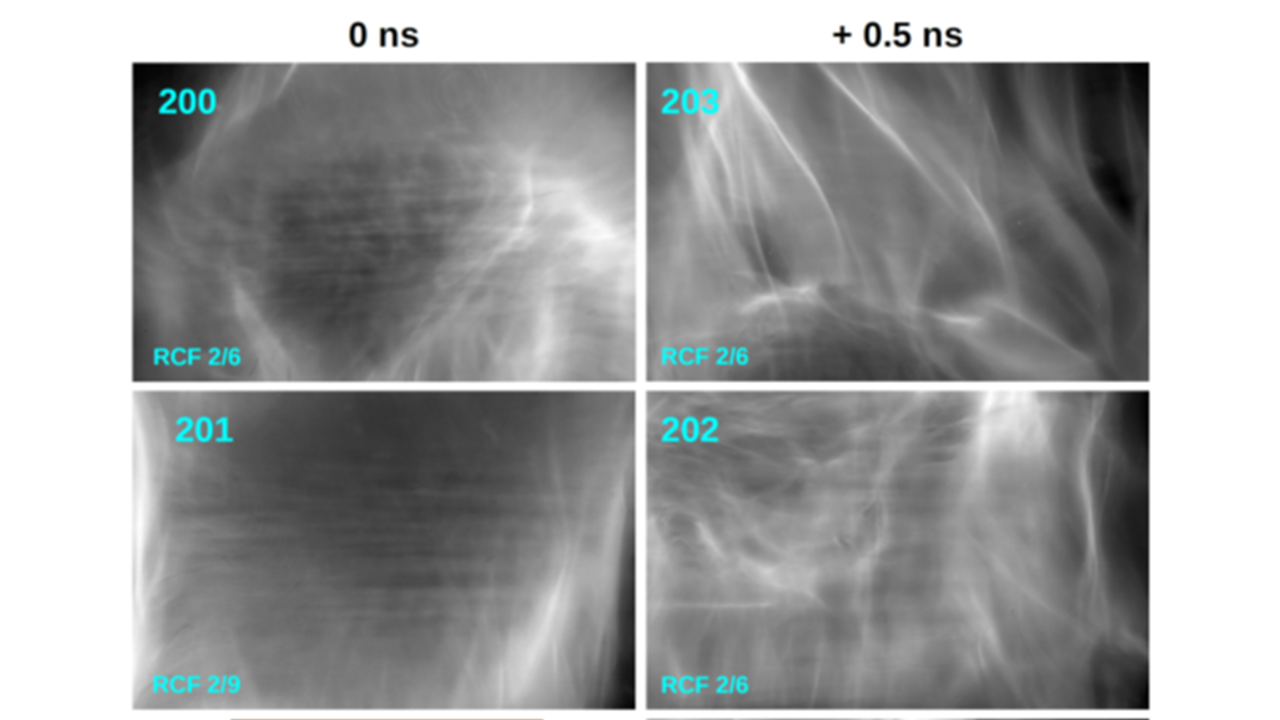
\includegraphics[width=0.45\textwidth]{rcf.png}
\caption{ \label{fig:xpfuchs_xp}  
(a) Sketch of the experimental setup.
(b) Experimental RCF (obtained using 3 MeV protons) from two shots of the LULI experiment, at $0$ and $0.75$ ns after the maximum intensity reaches the center of the plasma slab.  The scale indicated at the bottom of the image refers to the target plane. 
 }
\end{figure}
\begin{figure}
\begin{tabular}{cc}
(a) $T_e(t)$ and $I_0(t)$&
(b) $\Gamma \times L$  \\
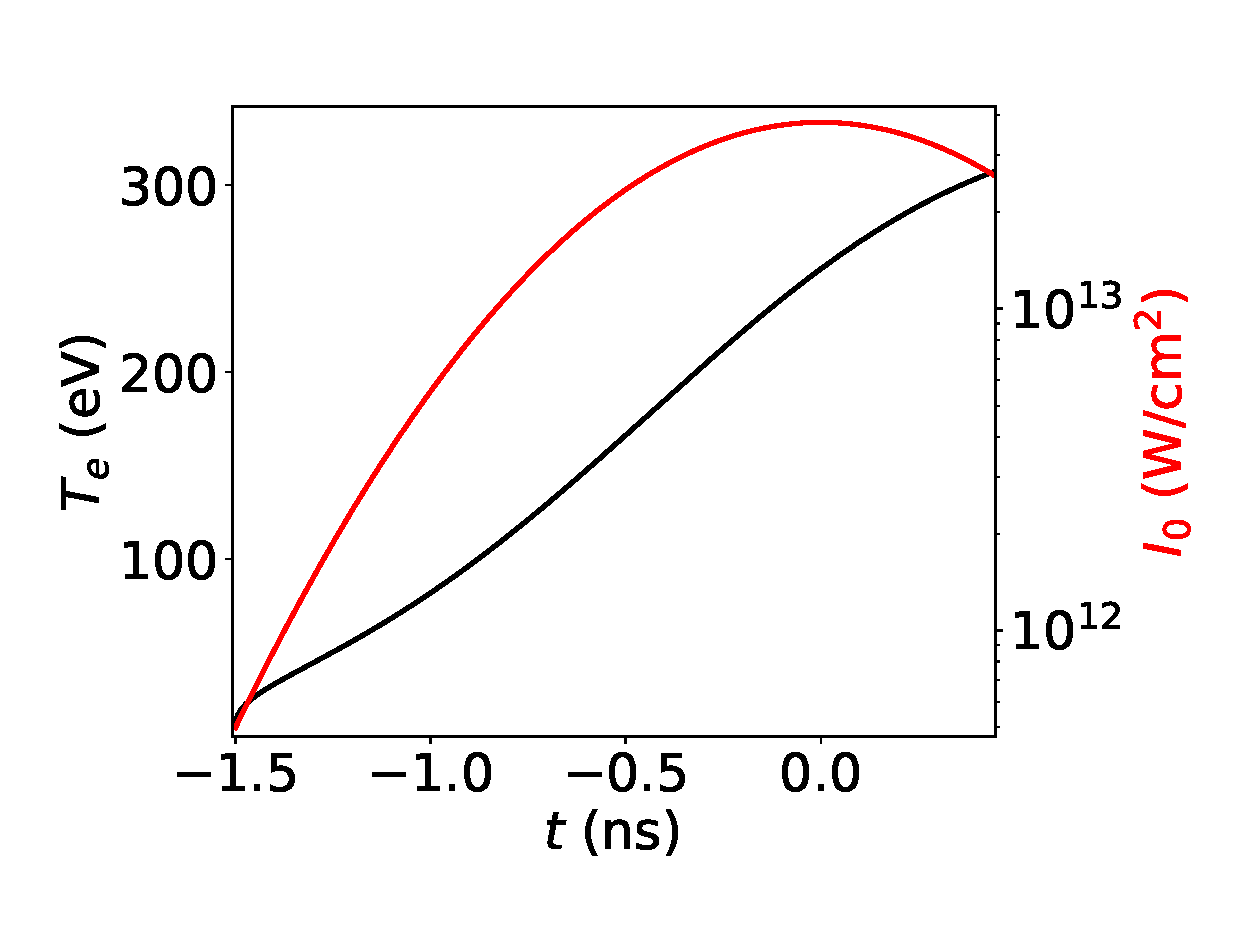
\includegraphics[width=0.24\textwidth]{xpFuchs_te.eps}& 
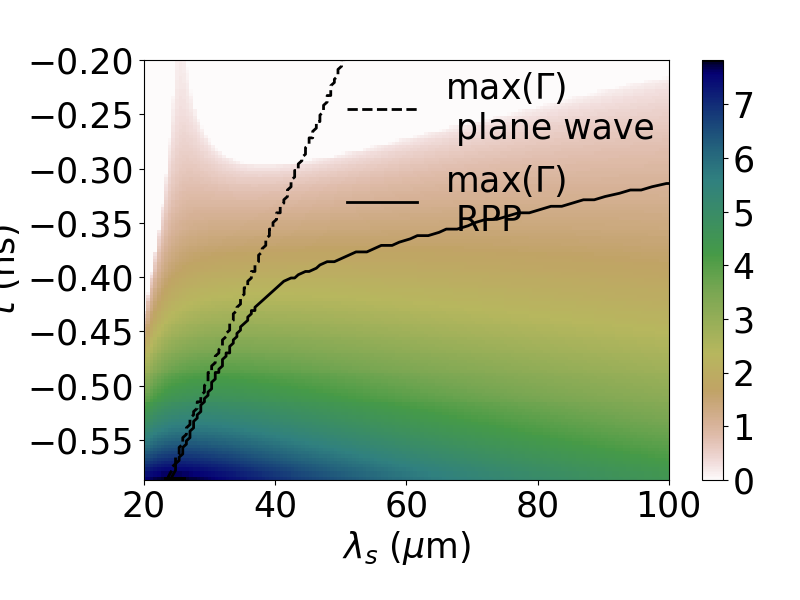
\includegraphics[width=0.24\textwidth]{xpFuchs.png}
\end{tabular}
\caption{ \label{fig:xpfuchs_th}  
(a) Temporal evolution of the electron temperature 
%from an Hydrodynamic simulation  \tc{with the code HERA} and 
from the resolution of $(3/2)n_e d_tT_e=\nu_BI_02^{-t^2/\tau^2}/c$ with $\tau = 600\,\rm ps$  and $T_e(-1.5 \, \rm{ns})=10\,\rm eV$ (left axis, black).
The intensity evolution is superimposed as a red line (right axis).
(b) Solution of Eq. \eqref{eq:dispe2polyrpp} normalized to the plasma length  $L$  for $v_\phi=0$ and in the fluid framework [Eq. \eqref{eq:alphaf}] with $I_0=3.8\times 10^{13}\, \rm W/cm^2$, $2\pi/k_0=1\,\rm\mu m$, $f_\sharp=11$, $Z_i=2$, $A=4$, $n_e=10^{19} \,\rm cm^{-3}$,  $L=1\,\rm mm$ and  $Z_iT_e/T_i=10$. 
The growth rate maximum is superimposed as a  black line in the RPP case and as a dashed line in the plane wave case [Eq. \eqref{eq:dispe2poly}].
 }
\end{figure}


A low temperature plasma may also be filamentation-unstable to the  propagation of an RPP pulse.
For a single ion species plasma, and provided $ZT_e\gg T_i$,   we recall that $\alpha_f(0)=1\simeq \alpha_k(0)$, for this reason, the filamentation growth coincides in both  kinetic and hydrodynamic frameworks. 
Hence, restricting, in this section, the analysis to the fluid plasma response, we aim at comparing our predictions with the laser filamentation observed experimentally at relatively low temperature and as measured by mean of the proton-radiographic techniques of a propagating RPP pulse.

The experiment detailed in Ref. \cite[]{PRL_Sarri_2011} uses a tightly focused ($f_\sharp =3$) RPP pulse,  therefore probably out of reach of our dispersion relations where we neglected diffraction  on the pump wave envelope [in Eq. \eqref{eq:erpp}].
Hence the choice has thus been made to lean on 
a longer focus  experiment performed using the LULI 100TW laser facility at the fundamental wavelength of 1.053 micron. The beam after amplification is split in several beams: a vacuum compressed beam (compressed beam in Fig. \ref{fig:xpfuchs_xp}(a)  350 fs) used for the production of protons as a diagnostic \cite{RSI_Mackinnon_2004}, and an interaction beam (interaction beam in Fig. \ref{fig:xpfuchs_xp}(a),  uncompressed, $\tau=600$ ps FWHM). All beams are horizontally polarized. As shown in 
Fig. \ref{fig:xpfuchs_xp}(a), both beams are focused at $90^o$. An optical time slide on one beam allowed to set a variable delay between B1 and B2 with sub-ps precision. B2 was focused, using an $f/24$ ($f=2.1$ m, $f_\sharp=24$)  lens coupled to a RPP, producing an intensity at focus of $I_0=3.8\times 10^{13}\, \rm W/cm^2$, onto a $L=1\,\rm mm$ diameter supersonic Helium jet corresponding to  $n_e/n_c\simeq 10^{-2}$ at full ionisation. 
Proton radiography of the interaction was performed using a laminar beam of protons generated by the compressed beam.
For this, it was focused (with a FWHM of $\sim 6$ microns) to a peak intensity of $4\times 10^{19}\, \rm W/cm^2$ on 10 microns thick Au foils positioned $d=3.5$ mm away from the center of the gas jet. This produced  \cite{PRL_Snavely_2000} a beam of laminar protons having a broad energy spectrum extending here from 0 to 15 MeV. The protons originate from hydrogenated contaminants on the target surface. They were detected downstream, at $D=43.5$ mm from the gas jet, by a stack radiochromic films (RCFs) \cite{Bolton_2014}  protected by a $14\, \rm \mu m$-thick Al range filter. This resulted in a magnification of the proton projection onto the RCFs of $M=(d+D)/d =13.1$. RCFs are preferentially sensitive to penetrating protons, which have a large specific energy-loss and produce a high contrast image; the stack arrangement therefore allowed a coarse resolution in proton energy (determined using the code SRIM \cite{Ziegler_2010}). 
The spatial resolution of the proton radiography is given by the virtual source size which is $\sim 5$ microns \cite{PRL_Cowan_2004} and the temporal resolution is given by the time required by the protons to cross the interaction zone, i.e. $\sim 4$ ps for $3$ MeV protons. The different time shown in Fig. \ref{fig:xpfuchs_xp}(b) corresponds to different shots. 

An estimate of the plasma temperature evolution may be obtained easily in this low temperature and low density experiment ($T_e\lesssim 300 \,\rm eV$, $n_e/n_c=10^{-2}$) by neglecting the electron thermal diffusion and accounting only for the inverse Bremsstrahlung laser absorption calculated on the transversely averaged intensity (neglecting the speckle-scale intensity fluctuations). The resulting electron temperature evolution, \mbox{$(3/2)n_e d_tT_e=\nu_BI_02^{-t^2/\tau^2}/c$} (where $\nu_B\propto T_e^{-3/2}$ is  the bremasstrahlung laser absorption coefficient) has been resolved and is illustrated in Fig. \ref{fig:xpfuchs_th}(a), showing that  $T_e\lesssim 150\, \rm eV $ is obtained half a nanosecond before the pulse maximum intensity, \emph{i.e.} for $I\lesssim 4\times 10^{12}\, \rm W/cm^2$. 
The colormap of Fig. \ref{fig:xpfuchs_th}(b) illustrates the RPP filamentation spatial  growth normalized to the plasma length  as a function of   wavelength and  time, for the experimental parameters and the  intensity and electron temperature evolution discussed above [see Fig. \ref{fig:xpfuchs_th}(a)].
Moreover, the RCF signal late-time evolution suggests a ratio  $Z_iT_e/T_i=5$ as discussed in appendix. Hence, the RPP growth rate maximum (black plain line) demonstrates that a reasonable gain is obtained,  $\Gamma L\gtrsim 3$, when $t\simeq -1.1\,\rm ns$, $I\sim 4\times 10^{12}\,\rm W/cm^2$ and  $T_e\lesssim 80\, \rm eV$.
As soon as $t>-0.8\, \rm ns$, the density fluctuations should cease growing as the gain drops below unity  and subsequently be damped by the Landau process over a few ($\gamma_0c_s2\pi/\lambda_s)^{-1} \sim 1\, \rm ns$.
This suggests that the filamentation grows and saturates rapidly before the most energetic part of the beam reaches the center of the gaz jet, leading to  density fluctuations of wavelength   $\lambda_F \sim 60 \,\rm\mu m$ and measurable for $t>0\,\rm ns$. The resulting electrostatic field is able to deflect the probing protons   causing the proton dose modulation illustrated in Fig \ref{fig:xpfuchs_xp}(b). 
The estimated experimental wavelength of $\simeq 77 \,\rm\mu m$, obtained by maximizing the Fourier transformed experimental signal over a central lineout, agrees correctly with our RPP dispersion relations (see Fig. \ref{fig:xpfuchs_ap}(a)  in appendix). 
Note that the textbook plane wave filamentation dispersion relations [Eq. \eqref{eq:dispe2poly} for $v_\phi=0$] predicts a  smaller dominant wavelength of $ \lambda_F\lesssim  35\, \rm\mu m$ (when $T_e\lesssim80\, \rm eV$), illustrated as a dashed black line in Fig. \ref{fig:xpfuchs_th}(b). A large disagreement of the  RPP and plane wave most unstable wavelengths is obtained when  $\lambda_s> f_\sharp\lambda_0=24\,\rm\mu m$ [in Fig. \ref{fig:xpfuchs_th}(b), as discussed in Sec. \ref{sec:filam}], demonstrating the significance of our random phase plate dispersion relations regarding realistic conditions.

\subsection{Forward Brillouin scattering of a  spatially smoothed beam}
Figures \ref{fig:disperpp} and \ref{fig:dispeCHrpp} shows also significant differences compared to the propagation of a plane wave  regarding the forward Brillouin scattering.  
Either Fluid or kinetic, for single or multiple ion species, 
the spatial growth rate appears much more peaked around $v_\phi\simeq c_s$ [or $v_\phi\simeq 0.8c_s$ for  the kinetic CH case, Fig. \ref{fig:dispeCHrpp}(a)] and the propagation of the RPP pulse more unstable  [$\Gamma/k_0\sim 0.1$, Fig.  \ref{fig:disperpp}(a) and Fig.  \ref{fig:dispeCHrpp}(a)]  than for a plane wave case  [$\Gamma/k_0\simeq 2 \times 10^{-4}$, Fig.  \ref{fig:dispe}(a)].
Therefore degrading the pump spatial coherence does subjugate the filamentation instability (or at least significantly reduces it for the CH-case), however, at the expense of favoring the the spatial growth of the forward Brillouin instability.
The forward scattering of an RPP beam ensues from the superposition of all the pulse spectral contributions, the final superposition of acoustic waves may be constructive or destructive depending on the wavevector direction and amplitude relative to the plasma resonance [characterized by $\alpha_{k/f}$, Eqs. \eqref{eq:alphak}-\eqref{eq:alphaf}]. 
As a consequence, the spatial growth consists in a succession of peaks aligned around $v_\phi\simeq c_s$ and spread from $\vert k_s\vert=0$ to a fraction of $k_0$. The separation of these peaks [a few $ 10^{-2}k_0$ for Fig. \ref{fig:disperpp}(a) and $\sim 10^{-1}k_0$ for \ref{fig:dispeCHrpp}(a)], depends on the propagation properties of the driven acoustic waves and the plasma response such as the width of the resonance. 
The factor $\alpha_{k/f}$ that  holds the acoustic waves propagation characteristics, contrasts  in the fluid and in the kinetic framework for $\vert v_\phi\vert>0$ and $Z_iT_e/T_i\lesssim 10$ thus explaining the disparities between Figs. \ref{fig:disperpp}(a) and (c) [as well as  \ref{fig:dispeCHrpp}(a) and (c)], such as the spectral distribution of the unstable clusters and the growth maximum. 
Figures \ref{fig:disperpp}(a,c) present a similar repartition of the unstable clusters with a somewhat larger value of the local  maximum for the kinetic calculations. 
For Figs. \ref{fig:dispeCHrpp}(a,c),
twice more unstable peaks are evidenced in the fluid  (c) than in the kinetic (a) framework, and apart from that,  surprisingly similar growth behavior are obtained, either in the single or multi ion species case. 

Regarding the propagation of an RPP pulse, the growth spectral width has to be compared with the  beam width in vacuum $k_m/k_0=1/(2f_\sharp) \simeq 0.062$.
For the H$^+$-plasma, 
the range  $0.05 \lesssim k/k_0\lesssim 0.4$ 
is unstable thus probably 
leading to the increase of the $f_\sharp$-cone 
angle from $1/(2f_\sharp)=3.6^o$ to $\sim 21^o$.
Hence, a large modification of the beam 
properties  could appear during its propagation thus affecting the energy deposition outcome.
Regarding the CH-plasma, one may notice that unlike for the single ion case, the peaks are located around $v_\phi=0.8c_s$, implying a lower acoustic frequency (than for the single ion species case or than the fluid calculations) and thus less red-shifting of the scattered wave.
Two and six unstable peaks are evidenced in Figs. \ref{fig:dispeCHrpp}(a) and (c), corresponding to $\sim (16^o,21^o)$ and $ \sim (8^o,11^o,14^o,17^o,19^o,21^o)$ scattering direction, respectively.
Albeit  a similar maximum growth rate  predicted by the kinetic and fluid calculations, different scattering directions are obtained which indicates that the fluid framework  suffers, in some cases, from an ill-forecast of the scatter spectral properties. 

\section{Comparison with hydrodynamic simulation}
In this section we aim at validating the derived fluid spatial growth rate through a  comparison with hydrodynamic simulations. Regarding the kinetic counterpart, the corresponding full "particle-in-cell" simulations are found to be out of reach of present super-computers and are therefore out of this manuscript scope. 

We thus performed two \textsc{hera} hydrodynamic simulations with a paraxial resolution of the RPP beam propagation \cite[]{Loiseau_2006}. 
A 2D domain of size $L_x \times L_y = 2000 \times 512\, \rm \mu$m$^2$ will be used. 
A RPP-beam  propagating in the $x$ direction was injected from the left boundary at $x_\mathrm{BC}=0$ with a  $\lambda_0=0.35\, \rm\mu m$-wavelength and an averaged intensity of $I_0=6\times 10^{14}\, \rm W/cm^2$.
The focal spot is located at the center of the simulation domain, $x_\mathrm{foc}=1000\, \rm \mu m$ with a focal number of $f_\sharp = 8$, and
{
a spatial and a temporal envelope following
\begin{align}
    \hat{g}(y) &= \exp(-\vert y\vert ^o/2\sigma_g^o)  \, ,  \label{eq:g}\\
    h(t) &= \mathrm{min}(t/\tau_h,1) \, ,\label{eq:h}
\end{align}
respectively with a $\tau_h=1\, \rm ps$,  $o=5$ and $\sigma_g = 200\,\rm \mu m$. }
For sake of simplicity and comparison purposes, the bremsstrahlung energy deposition is neglected and the non-local thermal correction of Eq. \eqref{eq:nl} is accounted for.  
Moreover a barotropic gas is assumed  with an electron density of $n_e =0.1n_c $ and outflow boundary for the fluid.
Use has been made of meshes of size $dx =0.325\,\rm \mu m$, $dy = 0.0625\, \rm \mu m$
%and a timestep of $dt=10^{-13}$ s 
with a Landau acoustic damping rate calculated on  Eq. \eqref{eq:g0} with the initial plasma parameters. 
The Landau damping acoustic operator is computed transversely to the laser direction in the Fourier space, as introduced in Ref. \cite[]{POP_Rose_96}, described in \cite[]{Berger_98} and used in   \cite{phd-PEML,Masson_2006,Huller_2008}.
In order to focus on the FSBS, we do no account for any back-scattering in our simulations. 

\begin{figure*}
\begin{tabular}{ccc}
(a) $\log_{10}(I \,[\mathrm{W.cm^{-2}}] )$&
(b) $\log_{10}(\vert\delta n_e(\omega,k_y,x_2)/n_c\vert^2)$ &
(c) $\Gamma/k_0$\\ 
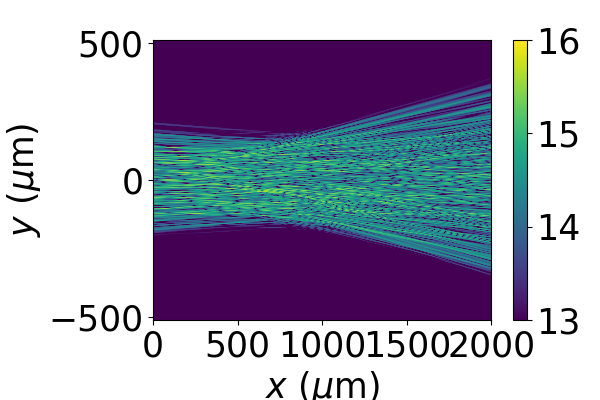
\includegraphics[width=0.3\textwidth]{I300eV_t65ps.png}
&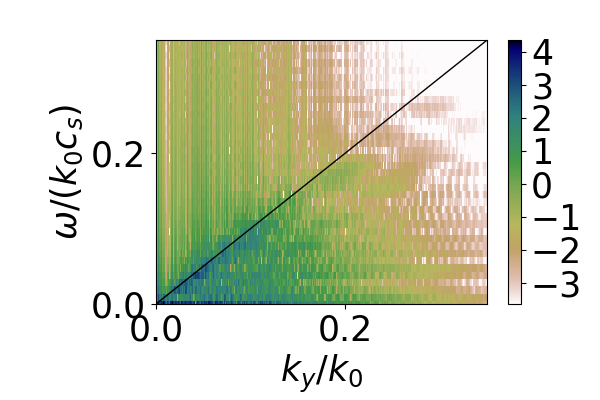
\includegraphics[width=0.3\textwidth]{dnwk_300eV.png}
&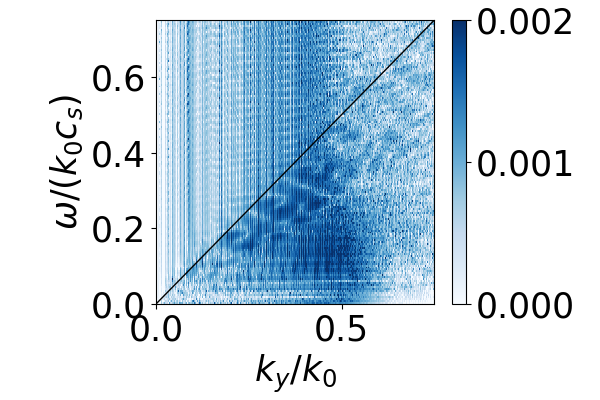
\includegraphics[width=0.3\textwidth]{G300eV.png}
\end{tabular}
\begin{tabular}{ccc}
(d) $\log_{10}(I \,[\mathrm{W.cm^{-2}}] )$&
(e) Theory &
(f) $\Gamma/k_0$\\ 
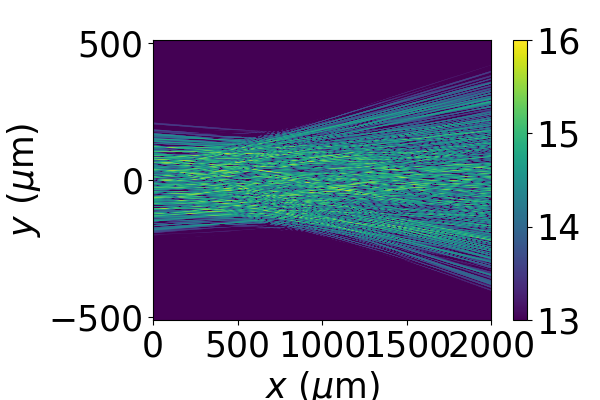
\includegraphics[width=0.3\textwidth]{I100eV_t65ps.png}
&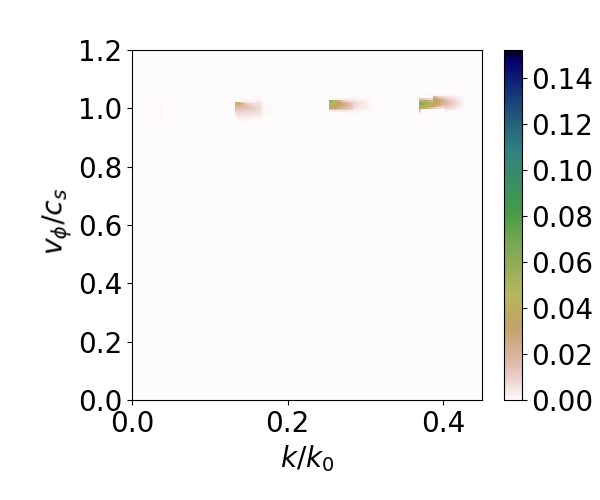
\includegraphics[width=0.25\textwidth]{gfH100eV.png}
&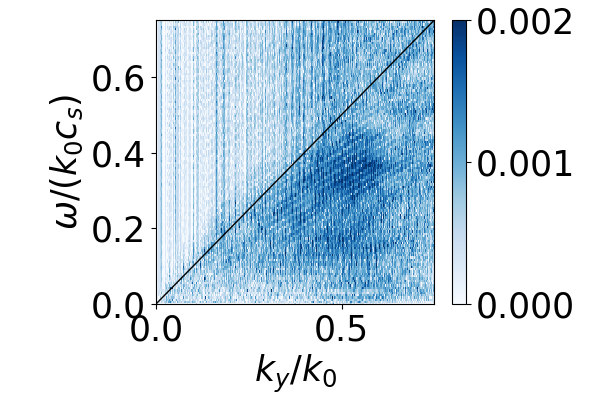
\includegraphics[width=0.3\textwidth]{G100eV.png}
\end{tabular}
%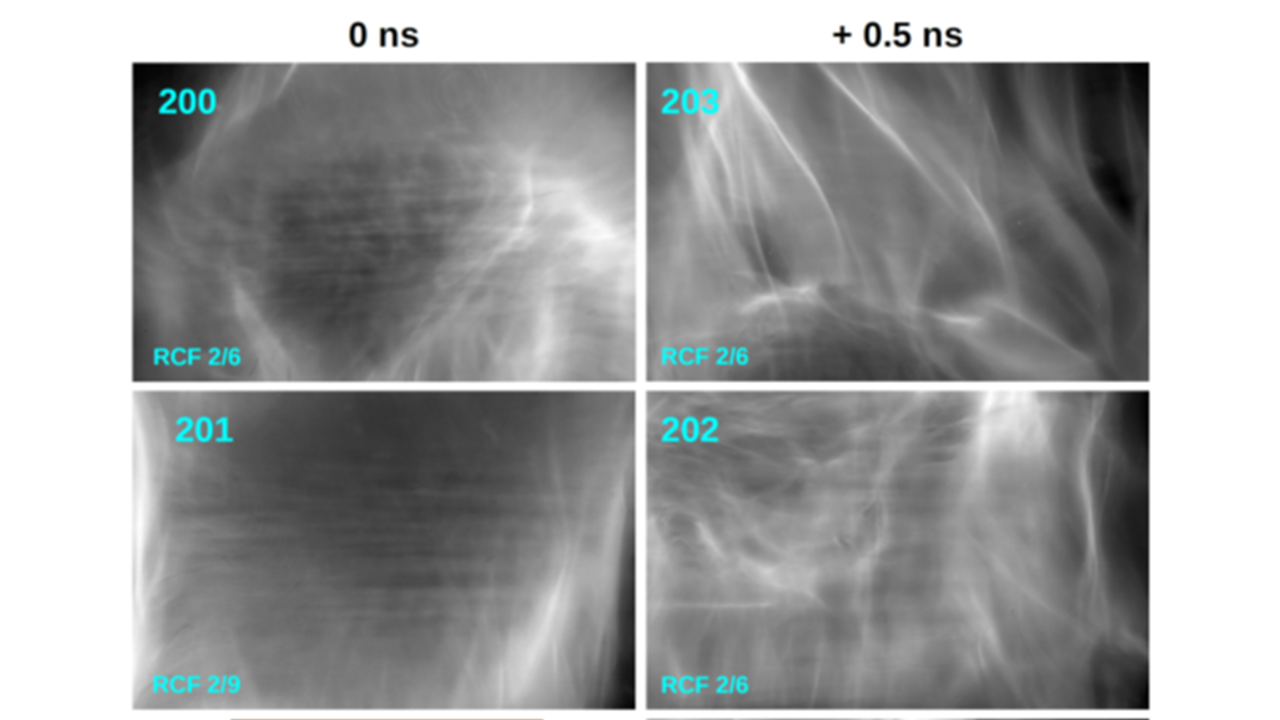
\includegraphics[width=0.5\textwidth]{rcf.png}
\caption{ \label{fig:comphydro}  Simulation results for the H$^+$ plasma with $n_e=0.1n_c$, $T_e=1\,\rm keV$ and $T_i=300\,\rm eV$ (a,b,c) and $T_i=100\,\rm eV$ (d,e).
(a,d) Intensity profile at $t=65\,\rm ps$ and (b) spatio-temporal spectrum at $x_2=250\,\rm\mu m$ of $\delta n_e(\omega,k_y,x_2)$. 
(c,f) Effective spatial growth rate extracted from the numerical results between $50$ and $200\,\rm ps$ following Eq. \eqref{eq:gammah} with $(x_1,x_2)=(100,250)\, \rm \mu m$.
The corresponding theoretical  growth rate as discussed in Sec. \ref{sec:diperpp} are illustrated in Fig. \ref{fig:disperpp}(c) and panel (e) for $Ti=300$ and  $100\, \rm eV$, respectively.
The acoustic eigenmode $\omega=k_yc_s$ is superimposed on (b,c,f) as black plain lines.}
\end{figure*}
As illustrated in Figs. \ref{fig:comphydro}(a,d),  the RPP beam presents a cone angle increase as soon as $x\gtrsim 500\,\rm\mu m$ at $t=65\,\rm ps$ (and later on). Due to the FSBS, its growth may be characterized and compared to our predictions. 

The   density fluctuation spectrum [Fig.  \ref{fig:comphydro}(b) for the case $T_i=300\,\rm eV$] is peaked along the acoustic mode ($\omega=k_yc_s$ as a black solid line) as expected. When looking at $k_y/k_0\gtrsim 0.2$, the acoustic trace seems to be broken down into clusters that vanishes for  $k_y/k_0\gtrsim 0.34$, qualitatively consistent with the FSBS growth illustrated in Fig. \ref{fig:disperpp}.
We also extracted an effective growth rate from our numerical results by proceeding to the spatial (in the $y$ direction) and temporal Fourier transform of two lineouts of the density fluctuations, at $x=x_1$ and $x_2$ and following,
\begin{equation}
    \Gamma = \frac{1}{2(x_2-x_1)} \ln \left[\frac{\vert \delta n_e(x_2,k_y,\omega)\vert^2}{\vert \delta n_e(x_1,k_y,\omega)\vert^2}\right] \,. \label{eq:gammah}
\end{equation}
Illustrated in Figs.  \ref{fig:comphydro}(c,f) for both cases $T_i=300$ and $100\, \rm eV$ in the plane $(\omega,k_y)$, no positive growth are evidenced for $\omega=0$, \emph{i.e.} no filamentation instability, consistently with the theoretical predictions and with Figs. \ref{fig:comphydro}(a,d). 
Interestingly, when looking at the acoustic trace, $\omega=k_yc_s$ (as black solid lines) in Fig. \ref{fig:comphydro}(c), a succession of peaks are evidence as predicted by our theory [Fig. \ref{fig:disperpp}(c)]. Their separation of $\sim 0.03 k_0$ is consistent with Fig. \ref{fig:disperpp}(c). Moreover, they extend from $k_y \sim  0.2k_0$  to $0.6k_0$, therefore exceeding the initial transverse spectral width of $k_0/2f_\sharp  \simeq 0.062k_0$ and  explaining the large cone angle   observed for $x>500\,\rm\mu m$ in Fig. \ref{fig:comphydro}(a) of $\sim 0.2k_0$ (\emph{i.e.} $11^o$).

Figure  \ref{fig:comphydro}(c) seems to  present  clusters located below the acoustic trace, $\omega <k_y c_s$. These features may correspond to the  nonlinear evolution of the growing FSBS acoustic perturbations propagating significantly off the $y$ direction, which, once projected on the $k_y$-Fourier axis, appear at sub-acoustic frequency levels. 
When $T_i=100\, \rm eV$, the theoretical predictions [Fig. \ref{fig:comphydro}(e)] yields only three unstable peaks located between $\sim 0.2k_0$ and $\sim 0.4k_0$. Hence, two faint clusters (for $k_y\ge 0.3k_0$) are evidenced in Fig. \ref{fig:comphydro}(f) which contrasts with the case $T_i=300\, \rm eV$.

Regarding the simulation growth level, the convective nature of the instability  addressed here complicates the isolation of the spatially growing and propagating  acoustic fluctuations and therefore, the accurate measurement of the exponential slope.   
However, we could pinpoint the instability growth over a $150\,\rm\mu m$-long window (between  $x_1=100\,\rm \mu m$  and $x_2=250\, \rm\mu m$) for $50\,\mathrm{ps}\le t\le200\,\mathrm{ps}$, 
a much larger distance than the typical  growth length of $1/\mathrm{max}(\Gamma)\sim 1\,\rm\mu m$.  
Hence, the validation of the  FSBS spatial growth has to settle for a good accordance of the space and time spectrum shape and the assessment of the  multi-unstable acoustic peaks  characterizing the FSBS of an RPP beam.
A better  understanding of the competition between the convective or absolute modes in the kinetic framework is required,   as studied  in Ref. \cite[]{phd-Grech,PRL_Grech_2009} for the fluid case  (see Ref. \cite[]{POP_Grismayer_2004}  regarding the stimulated Raman scattering) or  following   Ref. \cite[]{PR_Hall_68}.

\section{Conclusion}
The spatial growth of the  pump wave filamentation and of the forward Brillouin instabilities, as derived in this study, enables the comparison of both instabilities in the fluid and kinetic frameworks. They confirm the importance  of spatial smoothing techniques on the control of the laser filamentation and pinpoints that, in some cases such as multi-ion  or cold-enough  plasmas, this instability may survive.
Our dispersion relations demonstrate that, although hydrodynamic codes  predictions are correct regarding the description of the laser filamentation in a single-ion species plasmas,
the effective spatial growth rate is underestimated in the case of multi-ion plasmas. 
%Provided one accounts for multi-ion species effects and non-local thermal corrections, working in the fluid framework seems to be reasonable regarding the laser filamentation instability.
Moreover, we also conclude that the use of Random phase plates may further destabilize the laser propagation   regarding FSBS,  leading to larger angle scattering and thus stronger modification of the energy deposition.
Albeit some qualitative similarities between the hydrodynamic and kinetic predictions, the forward Brillouin scattering of an RPP pulse also brings to light the significance of the kinetic damping of  driven acoustic  waves able to  affect  the    scatter spectrum. 
The FSBS growth can be  greatly underestimated in hydrodynamic codes  even for moderate $Z_iT_e/T_i$-ratios leading to an imperfect description of the beam cone-angle increase and of  the plasma smoothing. 

In deriving the spatial growth of the forward instabilities, we neglected the transverse spatial laser envelope and its variations due to diffraction, hence, our results should remain valid in realistic conditions for large-enough and flat-enough focal spots and for long enough focus. Moreover,  our analytical results are averaged over the random phase plate elements thus failing to capture the corresponding  statistical fluctuations. 

The use of SSD, which  causes the so-called speckles to vanish and change position, is known  experimentally to significantly stabilize the pump propagation. The framework developed in this publication  allows the insertion of spectral dispersion in the dispersion relations of importance for LMJ or NIF like facilities  and is left for future work. Moreover, 
combining the results of  Ref. \cite[]{POP_Debayle_2019} with our spatial growth rates opens the way for 
including the RPP forward Brillouin scattering   in the vastly used ray tracing schemes, possibly greatly improving their prediction precision regarding high-energy laser experiments.
In addition, the impact of a flow on the growth of the FSBS is also of interest here. 
Finally, the comparison of our model with NIF or LMJ-relevant experiments is currently underway. 

\section*{Acknowledgements}
We acknowledge important discussions with M. Grech and L. Gremillet. We acknowledge the expert support of the LULI technical teams. We also admit the role of the lockdown following the COVID19 plague for forcing us to take the time to finalize this theoretical work. This work has been done under the auspices of CEA-DAM  and the simulations were performed using HPC resources at TGCC/CCRT and CEA-DAM/TERA.

\section*{Data availability}
The data that support the findings of this study are available from the corresponding authors upon reasonable request.

\appendix
\section*{Appendix: constraining $Z_iT_e/T_i$ in the experiment of Sec. \ref{sec:xp}}
\label{sec:ztesti}
\setcounter{equation}{0} 
\renewcommand{\theequation}{A\arabic{equation}}
\setcounter{figure}{0} 
\renewcommand{\thefigure}{A\arabic{figure}}
\begin{figure}
\begin{tabular}{cc}
(a) FFT of transverse lineout&
(b) Peak evolution\\
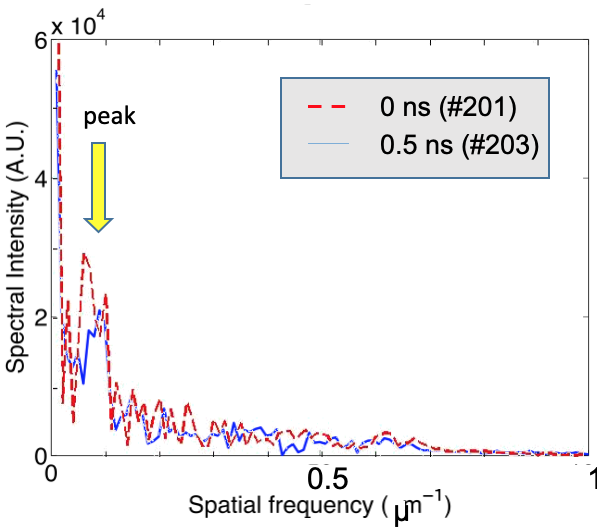
\includegraphics[width=0.24\textwidth]{fucshsfft.png}& 
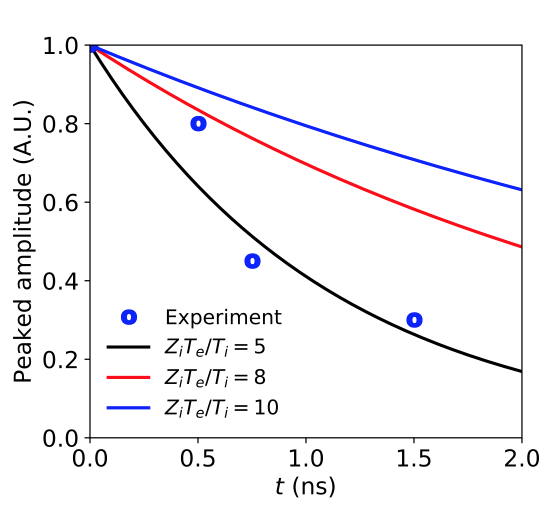
\includegraphics[width=0.22\textwidth]{fuchsztesti.png}
\end{tabular}
\caption{ \label{fig:xpfuchs_ap}  
(a) Fourier transforms of a central lineout across RCF similar as those shown in Fig. \ref{fig:xpfuchs_xp}(b), showing a peak at the dominant wavelength. Shown are two Fourier transforms corresponding to two different shots, taken at different times, as indicated.
(b) Peak temporal evolution [blue circles; these correspond to the amplitude of the peak observed in the Fourier transform identified by the yellow arrow in panel (a)]. Each point correspond to a different shot, where the time of the proton probing was changed with respect to the interaction laser propagating in the plasma [see examples of probing at two different time in  Fig. \ref{fig:xpfuchs_xp}(b)]. A decreasing exponential slope,  $\exp(-\nu t)$, is plotted for a Landau damping frequency given by $\nu=\gamma_0c_s2\pi/[77\,\rm\mu m]$ with the use of  Eq. \eqref{eq:g0} for a He$^{2+}$ plasma with $T_e=300\,\rm eV$ [see Fig. \ref{fig:xpfuchs_th}(a)] and various $Z_iT_e/T_i$.
}
\end{figure}
Figure \ref{fig:xpfuchs_ap}(a) shows the Fourier transform of a RCF transverse lineout pointing out a peak around a spatial frequency of  $2\pi/\lambda_s\sim 0.08\, \rm \mu m^{-1}$, \emph{i.e.} a wavelength of $\lambda_s \simeq 77\, \rm \mu m$.
Moreover, the comparison of the peak position at different times (blue plane line at $t=0\,\rm ns$ and red dashed line $t=0.5\,\rm ns$) demonstrates that the dominant wavelength stays mostly unchanged.  In that condition, and noting that the probing proton deflection results from an electric field and is therefore independent of the particle energy, the RCF dose modulation level depends mainly on the density fluctuations amplitude \cite[]{RSI_protograhyb}.
Hence, the peak temporal evolution of the experimental signal [blue circles in Fig. \ref{fig:xpfuchs_ap}(b)] correlates to the damping of the lingering acoustic waves, previously triggered by the filamentation instability over the first nanosecond of  the interaction beam.
In this low density configuration ($n_e/n_c\simeq10^{-2}$), 
we may therefore directly compare this decrease with an exponential slope, $\delta n_e \propto \exp(-\nu t)$ where $\nu = \gamma_0 c_s 2\pi/\lambda_s$ is the Landau damping acoustic rate. The calculations for a He$^{2+}$ plasma with $T_e=300\, \rm eV$ [as suggested by  Fig. \ref{fig:xpfuchs_th}(a)] and  for three different values of $Z_iT_e/T_i$ illustrated in  Fig. \ref{fig:xpfuchs_ap}(b) demonstrates that $Z_iT_e/T_i=5$ reproduces correctly the experimental data. 

\bibliography{biblio}
\end{document}
